% Options for packages loaded elsewhere
\PassOptionsToPackage{unicode}{hyperref}
\PassOptionsToPackage{hyphens}{url}
\PassOptionsToPackage{dvipsnames,svgnames,x11names}{xcolor}
%
\documentclass[
  letterpaper,
  DIV=11,
  numbers=noendperiod]{scrartcl}

\usepackage{amsmath,amssymb}
\usepackage{iftex}
\ifPDFTeX
  \usepackage[T1]{fontenc}
  \usepackage[utf8]{inputenc}
  \usepackage{textcomp} % provide euro and other symbols
\else % if luatex or xetex
  \usepackage{unicode-math}
  \defaultfontfeatures{Scale=MatchLowercase}
  \defaultfontfeatures[\rmfamily]{Ligatures=TeX,Scale=1}
\fi
\usepackage{lmodern}
\ifPDFTeX\else  
    % xetex/luatex font selection
\fi
% Use upquote if available, for straight quotes in verbatim environments
\IfFileExists{upquote.sty}{\usepackage{upquote}}{}
\IfFileExists{microtype.sty}{% use microtype if available
  \usepackage[]{microtype}
  \UseMicrotypeSet[protrusion]{basicmath} % disable protrusion for tt fonts
}{}
\makeatletter
\@ifundefined{KOMAClassName}{% if non-KOMA class
  \IfFileExists{parskip.sty}{%
    \usepackage{parskip}
  }{% else
    \setlength{\parindent}{0pt}
    \setlength{\parskip}{6pt plus 2pt minus 1pt}}
}{% if KOMA class
  \KOMAoptions{parskip=half}}
\makeatother
\usepackage{xcolor}
\setlength{\emergencystretch}{3em} % prevent overfull lines
\setcounter{secnumdepth}{-\maxdimen} % remove section numbering
% Make \paragraph and \subparagraph free-standing
\ifx\paragraph\undefined\else
  \let\oldparagraph\paragraph
  \renewcommand{\paragraph}[1]{\oldparagraph{#1}\mbox{}}
\fi
\ifx\subparagraph\undefined\else
  \let\oldsubparagraph\subparagraph
  \renewcommand{\subparagraph}[1]{\oldsubparagraph{#1}\mbox{}}
\fi


\providecommand{\tightlist}{%
  \setlength{\itemsep}{0pt}\setlength{\parskip}{0pt}}\usepackage{longtable,booktabs,array}
\usepackage{calc} % for calculating minipage widths
% Correct order of tables after \paragraph or \subparagraph
\usepackage{etoolbox}
\makeatletter
\patchcmd\longtable{\par}{\if@noskipsec\mbox{}\fi\par}{}{}
\makeatother
% Allow footnotes in longtable head/foot
\IfFileExists{footnotehyper.sty}{\usepackage{footnotehyper}}{\usepackage{footnote}}
\makesavenoteenv{longtable}
\usepackage{graphicx}
\makeatletter
\def\maxwidth{\ifdim\Gin@nat@width>\linewidth\linewidth\else\Gin@nat@width\fi}
\def\maxheight{\ifdim\Gin@nat@height>\textheight\textheight\else\Gin@nat@height\fi}
\makeatother
% Scale images if necessary, so that they will not overflow the page
% margins by default, and it is still possible to overwrite the defaults
% using explicit options in \includegraphics[width, height, ...]{}
\setkeys{Gin}{width=\maxwidth,height=\maxheight,keepaspectratio}
% Set default figure placement to htbp
\makeatletter
\def\fps@figure{htbp}
\makeatother

\usepackage{lineno}
\linenumbers
\usepackage[font={footnotesize, sf}, labelfont=bf, margin=0.05\linewidth]{caption}
\renewcommand{\familydefault}{\sfdefault}
% Bold the 'Figure #' in the caption and separate it from the title/caption
% with a period
% Captions will be left justified
\usepackage[
	aboveskip=1pt,
	labelfont=bf,
	labelsep=period,
	justification=raggedright,
	singlelinecheck=off
]{caption}

% Add numbered lines
\usepackage{lineno}
\linenumbers

% Package to include multiple title pages
% This will allow me to add a tile to the main text and to the SI
\usepackage{titling}

% Define command to begin the supplementary section
\newcommand{\beginsupplement}{
\setcounter{section}{0} % Restart section counter
\renewcommand{\thesection}{S\arabic{section}}%
\setcounter{table}{0} % Restart table counter
\renewcommand{\thetable}{S\arabic{table}}%
\setcounter{figure}{0} % Restart figure counter
\renewcommand{\thefigure}{S\arabic{figure}}%
\setcounter{equation}{0} % Restart equation counter
\renewcommand{\theequation}{S\arabic{equation}}%
}

% Add author affiliations
\usepackage{authblk}

\KOMAoption{captions}{tableheading}
\makeatletter
\makeatother
\makeatletter
\makeatother
\makeatletter
\@ifpackageloaded{caption}{}{\usepackage{caption}}
\AtBeginDocument{%
\ifdefined\contentsname
  \renewcommand*\contentsname{Table of contents}
\else
  \newcommand\contentsname{Table of contents}
\fi
\ifdefined\listfigurename
  \renewcommand*\listfigurename{List of Figures}
\else
  \newcommand\listfigurename{List of Figures}
\fi
\ifdefined\listtablename
  \renewcommand*\listtablename{List of Tables}
\else
  \newcommand\listtablename{List of Tables}
\fi
\ifdefined\figurename
  \renewcommand*\figurename{Figure}
\else
  \newcommand\figurename{Figure}
\fi
\ifdefined\tablename
  \renewcommand*\tablename{Table}
\else
  \newcommand\tablename{Table}
\fi
}
\@ifpackageloaded{float}{}{\usepackage{float}}
\floatstyle{ruled}
\@ifundefined{c@chapter}{\newfloat{codelisting}{h}{lop}}{\newfloat{codelisting}{h}{lop}[chapter]}
\floatname{codelisting}{Listing}
\newcommand*\listoflistings{\listof{codelisting}{List of Listings}}
\makeatother
\makeatletter
\@ifpackageloaded{caption}{}{\usepackage{caption}}
\@ifpackageloaded{subcaption}{}{\usepackage{subcaption}}
\makeatother
\makeatletter
\@ifpackageloaded{tcolorbox}{}{\usepackage[skins,breakable]{tcolorbox}}
\makeatother
\makeatletter
\@ifundefined{shadecolor}{\definecolor{shadecolor}{rgb}{.97, .97, .97}}
\makeatother
\makeatletter
\makeatother
\makeatletter
\makeatother
\ifLuaTeX
  \usepackage{selnolig}  % disable illegal ligatures
\fi

% References
% \usepackage[]{biblatex}
\usepackage[
	backend=bibtex,
	style=phys, 
	sorting=none,				% Do not sort bibliography
	url=false, 					% Do not show url in reference
	doi=false, 					% Do not show doi in reference
	isbn=false, 				% Do not show isbn link in reference
	eprint=false, 			% Do not show eprint link in reference
	maxbibnames=9, 			% Include up to 9 names in citation
	firstinits=true,
]{biblatex}
\addbibresource{references.bib}


\IfFileExists{bookmark.sty}{\usepackage{bookmark}}{\usepackage{hyperref}}
\IfFileExists{xurl.sty}{\usepackage{xurl}}{} % add URL line breaks if available
\urlstyle{same} % disable monospaced font for URLs
\hypersetup{
  pdfauthor={Manuel Razo-Mejia; Madhav Mani; Dmitri Petrov},
  pdfkeywords={bayesian inference, variational inference, relative
fitness, open-source, reproducible research},
  colorlinks=true,
  linkcolor={blue},
  filecolor={Maroon},
  citecolor={Blue},
  urlcolor={Blue},
  pdfcreator={LaTeX via pandoc}}

% Title
\title{Bayesian inference of relative fitness on high-throughput pooled competition assays}

% Authors
\author[1]{Manuel Razo-Mejia}
\author[2,3]{Madhav Mani}
\author[1,4,*]{Dmitri Petrov}

% Affiliations
\affil[1]{Department of Biology, Stanford University, Stanford, CA, USA}
\affil[2]{Department of Engineering Sciences and Applied Mathematics, Northwestern University, Chicago, IL, USA}
\affil[3]{NSF-Simons Center for Quantitative Biology, Northwestern University, Chicago, IL, USA}
\affil[4]{Stanford Cancer Institute, Stanford University School of Medicine, Stanford, CA, USA}
\affil[*]{Correspondence: dpetrov@stanford.edu}

\setcounter{Maxaffil}{0}
% Set affiliations in small font
\renewcommand\Affilfont{\itshape\small}

\date{}

\begin{document}
\ifdefined\Shaded\renewenvironment{Shaded}{\begin{tcolorbox}[borderline west={3pt}{0pt}{shadecolor}, sharp corners, frame hidden, interior hidden, enhanced, breakable, boxrule=0pt]}{\end{tcolorbox}}\fi

% Remove main text from the table of contents by specifying not to include
% any section or subsection
\addtocontents{toc}{\protect\setcounter{tocdepth}{-1}}


% Define reference segment for main text
\begin{refsegment}
% Generate filter to not include references from main text in the
% supplemental references
\defbibfilter{notother}{not segment=\therefsegment}

\maketitle

\begin{abstract}
    The tracking of lineage frequencies via DNA barcode sequencing enables the
  quantification of microbial fitness. However, experimental noise coming from
  biotic and abiotic sources complicates the computation of a reliable
  inference. We present a Bayesian pipeline to infer relative microbial fitness
  from high-throughput lineage tracking assays. Our model accounts for multiple
  sources of noise and propagates uncertainties throughout all parameters in a
  systematic way. Furthermore, using modern variational inference methods based
  on automatic differentiation, we are able to scale the inference to a large
  number of unique barcodes. We extend this core model to analyze
  multi-environment assays, replicate experiments, and barcodes linked to
  genotypes. On simulations, our method recovers known parameters within
  posterior credible intervals. This work provides a generalizable Bayesian
  framework to analyze lineage tracking experiments. The accompanying
  open-source software library enables the adoption of principled statistical
  methods in experimental evolution.
\end{abstract}

\hypertarget{introduction}{%
\section{Introduction}\label{introduction}}

The advent of DNA barcoding---the ability to uniquely identify cell
lineages with DNA sequences integrated at a specific locus---and
high-throughput sequencing has opened new venues for understanding
microbial evolutionary dynamics with an unprecedented level of temporal
resolution \autocite{levy2015,nguyenba2019a,ascensao2023}. These
experimental efforts rely on our ability to reliably infer the relative
fitness of an ensemble of diverse genotypes. Moreover, inferring these
fitness values over an ensemble of environmental conditions can help us
determine the phenotypic diversity of a rapid adaptation process
\autocite{kinsler2020}.

As with any other sequencing-based quantification, tracking lineages via
DNA barcode sequencing is inexorably accompanied by noise sources coming
from experimental manipulation of the microbial cultures, DNA
extraction, and sequencing library preparation that involves multiple
rounds of PCR amplification, and the sequencing process itself. Thus,
accounting for the uncertainty when inferring the relevant parameters
from the data is a crucial step to draw reliable conclusions. Bayesian
statistics presents a paradigm by which one can account for all known
sources of uncertainty in a principled way \autocite{eddy2004a}. This,
combined with the development of modern Markov Chain Monte Carlo
sampling algorithms \autocite{betancourt2017} and approximate
variational approaches \autocite{kucukelbir2016} have boosted a
resurgence of Bayesian methods in different fields
\autocite{efron2013a}.

We present a Bayesian inference pipeline to quantify the uncertainty
about the parametric information we can extract from high-throughput
competitive fitness assays given a model of the data generation process
and experimental data. In these assays, the fitness of an ensemble of
genotypes is determined relative to a reference genotype
\autocite{kinsler2020,ascensao2023}. Figure~\ref{fig-01}(A) shows a
schematic of the experimental procedure in which an initial pool of
barcoded strains are mixed with a reference strain and inoculated into
fresh media. After some time---usually, enough time for the culture to
saturate---an aliquot is transferred to fresh media, while the remaining
culture is used for DNA sequencing of the lineage barcodes. The
time-series information of the relative abundance of each lineage, i.e.,
the barcode frequency depicted in Figure~\ref{fig-01}(B), is used to
infer the relative fitness---the growth advantage on a per-cycle
basis---for each lineage with respect to the reference strain. The
proposed statistical model accounts for multiple sources of uncertainty
when inferring the lineages' relative fitness values (see
Section~\ref{sec-experiment} for details on sources of uncertainty
accounted for by the model). Furthermore, minor changes to the core
statistical model allow us to account for relevant experimental
variations of these competition assays. More specifically, in
Section~\ref{sec-multienv}, we present a variation of the statistical
model to infer fitness on growth dilution cycles in multiple
environments with proper error propagation. Furthermore, as described in
Section~\ref{sec-replicates}, our statistical model can account for
batch-to-batch differences when jointly analyzing multiple experimental
replicates using a Bayesian hierarchical model. Finally, a variant of
these hierarchical models, presented in Section~\ref{sec-genotypes}, can
account for variability within multiple barcodes mapping to equivalent
genotypes within the same experiment.

For all the model variations presented in this paper, we benchmark the
ability of our pipeline to infer relative fitness parameters against
synthetic data generated from logistic growth simulations with added
random noise. A \texttt{Julia} package accompanies the present method to
readily implement the inference pipeline with state-of-the-art
scientific computing software.

\hypertarget{results}{%
\section{Results}\label{results}}

\hypertarget{sec-experiment}{%
\subsection{Experimental setup}\label{sec-experiment}}

The present work is designed to analyze time-series data of relative
abundance of multiple microbial lineages uniquely identified by a DNA
barcode \autocite{kinsler2020,ascensao2023}. In these competition
assays, an ensemble of genotypes is pooled together with an unlabeled
reference strain that, initially, represents the vast majority
(\(\geq 90\%\)) of the cells in the culture (see schematic in
Figure~\ref{fig-01}(A)). Furthermore, a fraction of labeled genotypes
equivalent to the unlabeled reference strain---hereafter defined as
\emph{neutral} lineages---are spiked in at a relatively high abundance
(\(\approx 3-5\%\)). The rest of the culture is left for the ensemble of
genotypes of interest.

To determine the relative fitness of the ensemble of genotypes, a series
of growth-dilution cycles are performed on either a single or multiple
environments. In other words, the cultures are grown for some time;
then, an aliquot is inoculated into fresh media for the next growth
cycle. This process is repeated for roughly 4-7 cycles, depending on the
initial abundances of the mutants and their relative growth rates. The
DNA barcodes are sequenced at the end of each growth cycle to quantify
the relative abundance of each of the barcodes. We point the reader to
\textcite{kinsler2020} for specific details on these assays for \emph{S.
cerevisiae} and to \textcite{ascensao2023} for equivalent assays for
\emph{E. coli}. Figure~\ref{fig-01}(B) presents a typical barcode
trajectory where the black trajectories represent the so-called
\emph{neutral lineages}, genetically equivalent to the untagged ancestor
strain that initially dominates the culture. These spiked-in neutral
lineages simplify the inference problem since the fitness metric of all
relevant barcodes is quantified with respect to these barcodes---thus
referred to as \emph{relative fitness}.

\begin{figure}

{\centering 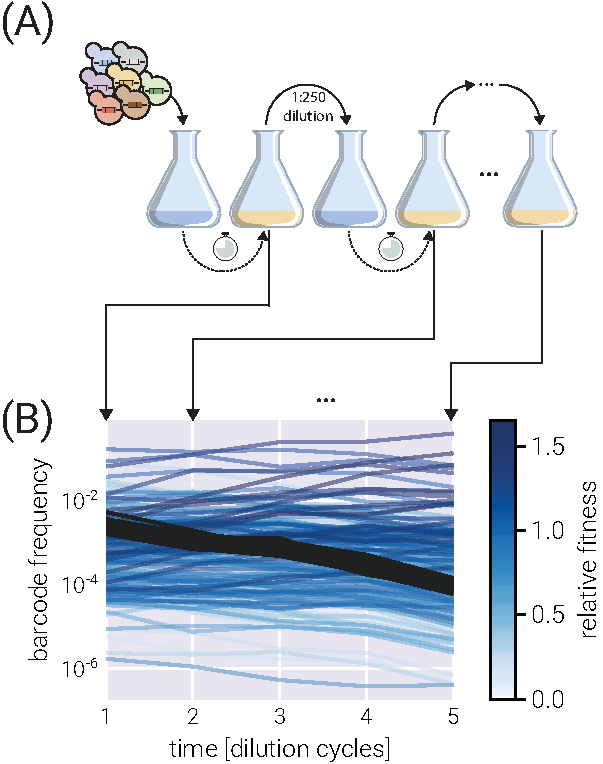
\includegraphics{./figs/fig01.pdf}

}

\caption{\label{fig-01}\textbf{Typical competitive fitness experiment}.
(A) Schematic of the typical experimental design to determine the
competitive fitness of an ensemble of barcoded genotypes. Genotypes are
pooled together and grown over multiple growth-dilution cycles. At the
end of each cycle, a sample is processed to generate a library for
amplicon sequencing. (B) Typical barcode trajectory dataset. From each
time point, the relative frequency of each barcode is determined from
the total number of reads. Shades of blue represent different relative
fitness. Darker gray lines define the typical trajectory of neutral
lineages.}

\end{figure}

\hypertarget{preliminaries-on-mathematical-notation}{%
\subsection{Preliminaries on mathematical
notation}\label{preliminaries-on-mathematical-notation}}

Before jumping directly into the Bayesian inference pipeline, let us
establish the mathematical notation used throughout this paper. We
define (column) vectors as underlined lowercase symbols such as
\begin{equation}\protect\hypertarget{eq-vec_def}{}{
\underline{x} = \begin{bmatrix}
    x_1\\
    x_2\\
    \vdots\\
    x_N
\end{bmatrix}.
}\label{eq-vec_def}\end{equation} In the same way, we define matrices as
double-underline uppercase symbols such as
\begin{equation}\protect\hypertarget{eq-mat_def}{}{
\underline{\underline{A}} =
\begin{bmatrix}
    A_{11} & A_{12} & \cdots & A_{1N}\\
    A_{21} & A_{22} & \cdots & A_{2N}\\
    \vdots & \vdots & \ddots & \vdots\\
    A_{M1} & A_{M2} & \cdots & A_{MN}\\
\end{bmatrix}.
}\label{eq-mat_def}\end{equation}

\hypertarget{sec-fitness_model}{%
\subsection{Fitness model}\label{sec-fitness_model}}

Empirically, each barcode frequency trajectory follows an exponential
function of the form \autocite{levy2015,kinsler2020,ascensao2023}
\begin{equation}\protect\hypertarget{eq-fitness}{}{
f_{t+1}^{(b)} = f_{t}^{(b)} \mathrm{e}^{(s^{(b)} - \bar{s}_t)\tau},
}\label{eq-fitness}\end{equation} where \(f_{t}^{(b)}\) is the frequency
of barcode \(b\) at the end of cycle number \(t\), \(s^{(b)}\) is the
relative fitness with respect to the reference strain---the quantity we
want to infer from the data---\(\bar{s}_t\) is the mean fitness of the
culture at the end of cycle number \(t\), and \(\tau\) is the time pass
between cycle \(t\) and \(t+1\). We can rewrite
Equation~\ref{eq-fitness} as
\begin{equation}\protect\hypertarget{eq-logfreq}{}{
\frac{1}{\tau}\ln \frac{f_{t+1}^{(b)}}{f_{t}^{(b)}} = (s^{(b)} - \bar{s}_t).
}\label{eq-logfreq}\end{equation} Equation~\ref{eq-logfreq} separates
the measurements---the barcode frequencies---from the unobserved
(sometimes referred to as latent) parameters we want to infer from the
data---the population mean fitness and the barcode relative fitness.
This is ultimately the functional form used in our inference pipeline.
Therefore, the relative fitness is computed by knowing the log frequency
ratio of each barcode throughout the growth-dilution cycles.

The presence of the neutral lineages facilitates the determination of
the population mean fitness value \(\bar{s}_t\). Since every relative
fitness is determined relative to the neutral lineage that dominates the
culture, we define their fitness to be \(s^{(n)} = 0\), where the
superscript \((n)\) specifies their neutrality. This means that
Equation~\ref{eq-logfreq} for a neutral lineage takes the simpler form
\begin{equation}\protect\hypertarget{eq-logfreq_neutral}{}{
\frac{1}{\tau}\ln \frac{f_{t+1}^{(n)}}{f_{t}^{(n)}} = - \bar{s}_t.
}\label{eq-logfreq_neutral}\end{equation} Therefore, we can use the data
from these reference barcodes to directly infer the value of the
population mean fitness.

It is important to notice that the frequencies \(f_{t}^{(b)}\) are not
the allele frequencies in the population (most of the culture is not
sequenced since the reference strain is not barcoded), but rather the
relative frequencies in the total number of sequencing reads. A way to
conceptualize this subtle but important point is to assume exponential
growth in the \emph{number of cells} \(N_t^{(b)}\) of the form
\begin{equation}\protect\hypertarget{eq-ncells}{}{
N_{t+1}^{(b)} = N_{t}^{(b)} \mathrm{e}^{\lambda^{(b)}\tau},
}\label{eq-ncells}\end{equation} for every barcode \(b\) with growth
rate \(\lambda^{(b)}\). However, when we sequence barcodes, we do not
directly measure the number of cells, but some number of reads
\(r_t^{(b)}\) that map to barcode \(b\). In the simplest possible
scenario, we assume \begin{equation}\protect\hypertarget{eq-r_to_n}{}{
r_{t}^{(b)} \propto N_{t}^{(b)},
}\label{eq-r_to_n}\end{equation} where, importantly, the proportionality
constant depends on the total number of reads for the library for cycle
\(t\), which might vary from library to library. Therefore, to compare
the number of reads between libraries at different time points, we must
normalize the number of reads to the same scale. The simplest form is to
define a relative abundance, i.e., a frequency with respect to the total
number of reads, \begin{equation}\protect\hypertarget{eq-r_to_n_norm}{}{
f_{t}^{(b)} \equiv \frac{r_{t}^{(b)}}{\sum_{b'} r_{t}^{(b')}}.
}\label{eq-r_to_n_norm}\end{equation} This is the frequency
Equation~\ref{eq-fitness} describes.

Our ultimate objective is to infer the relative fitness \(s^{(b)}\) for
each of the \(M\) relevant barcodes in the experiment---hereafter
referred to as \(s^{(m)}\) to distinguish from the general \(s^{(b)}\)
and the neutral lineages \(s^{(n)}\) relative fitness. To do so, we
account for the three primary sources of uncertainty in our model:

\begin{enumerate}
\def\labelenumi{\arabic{enumi}.}
\tightlist
\item
  Uncertainty in the determination of frequencies. Our model relates
  frequencies between adjacent growth-dilution cycles to the fitness of
  the corresponding strain. However, we do not directly measure
  frequencies. Instead, our data for each barcode consists of a length
  \(T\) vector of counts \(\underline{r}^{(b)}\) for each of the \(T\)
  cycles in which the measurements were taken.
\item
  Uncertainty in the value of the population mean fitness. We define
  neutral lineages to have fitness \(s^{(n)} = 0\), helping us anchor
  the value of the population mean fitness \(\bar{s}_t\) for each pair
  of adjacent growth cycles. Moreover, we take this parameter as an
  empirical parameter to be obtained from the data, meaning that we do
  not impose a functional form that relates \(\bar{s}_t\) to
  \(\bar{s}_{t+1}\). Thus, we must infer the \(T-1\) values of this
  population mean fitness with their uncertainty that must be propagated
  to the value of the mutants' relative fitness.
\item
  Uncertainty in each of the mutants' fitness values.
\end{enumerate}

To account for all these sources of uncertainty in a principled way, in
the next section, we develop a Bayesian inference pipeline.

\hypertarget{sec-bayesian_inference}{%
\subsection{Bayesian inference}\label{sec-bayesian_inference}}

As defined in Section~\ref{sec-fitness_model}, our ultimate objective is
to infer the vector of relative fitness values
\begin{equation}\protect\hypertarget{eq-fitness_mut_vec}{}{
\underline{s}^M = (s^{(1)}, s^{(2)}, \ldots, s^{(M)})^\dagger,
}\label{eq-fitness_mut_vec}\end{equation} where \(^\dagger\) indicates
the transpose. Our data consists of an \(T \times B\) matrix
\(\underline{\underline{R}}\), where \(B = M + N\) is the number of
unique barcodes given by the sum of the number of unique, relevant
barcodes we care about, \(M\), and the number of unique neutral
barcodes, \(N\), and \(T\) is the number of growth cycles where
measurements were taken. The data matrix is then of the form
\begin{equation}\protect\hypertarget{eq-R_mat}{}{
\underline{\underline{R}} = \begin{bmatrix}
- & \underline{r}_1 & - \\
- & \underline{r}_2 & - \\
 & \vdots & \\
- & \underline{r}_T & - \\
\end{bmatrix},
}\label{eq-R_mat}\end{equation} where each row \(\underline{r}_t\) is a
\(B\)-dimensional array containing the raw barcode counts at cycle
\(t\). We can further split each vector \(\underline{r}_t\) into two
vectors of the form
\begin{equation}\protect\hypertarget{eq-r-vec_split}{}{
\underline{r}_t = \begin{bmatrix}
\underline{r}_t^{N} \\
\underline{r}_t^{M}
\end{bmatrix},
}\label{eq-r-vec_split}\end{equation} i.e., the vector containing the
neutral lineage barcode counts \(\underline{r}_t^{N}\) and the
corresponding vector containing the mutant barcode counts
\(\underline{r}_t^{M}\). Following the same logic, matrix
\(\underline{\underline{R}}\) can be split into two matrices as
\begin{equation}\protect\hypertarget{eq-R-mat_split}{}{
\underline{\underline{R}} = \left[ 
\underline{\underline{R}}^N \; \underline{\underline{R}}^M
\right],
}\label{eq-R-mat_split}\end{equation} where
\(\underline{\underline{R}}^N\) is a \(T \times N\) matrix with the
barcode reads time series for each neutral lineage and
\(\underline{\underline{R}}^M\) is the equivalent \(T \times M\) matrix
for the non-neutral lineages.

Our objective is to compute the joint probability distribution for all
relative fitness values given our data. We can express this joint
posterior distribution using Bayes theorem as
\begin{equation}\protect\hypertarget{eq-bayes_obj}{}{
\pi(\underline{s}^M \mid \underline{\underline{R}}) = \frac{
\pi(\underline{\underline{R}} \mid \underline{s}^M) 
\pi(\underline{s}^M)}
{\pi(\underline{\underline{R}})},
}\label{eq-bayes_obj}\end{equation} where hereafter \(\pi(\cdot)\)
defines a probability density function. When defining our statistical
model, we need not to focus on the denominator on the right-hand side of
Equation~\ref{eq-bayes_obj}. Thus, we can write
\begin{equation}\protect\hypertarget{eq-bayes_obj_propto}{}{
\pi(\underline{s}^M \mid \underline{\underline{R}}) \propto
\pi(\underline{\underline{R}} \mid \underline{s}^M) 
\pi(\underline{s}^M).
}\label{eq-bayes_obj_propto}\end{equation} However, when implementing
the model computationally, the normalization constant on the right-hand
side of Equation~\ref{eq-bayes_obj} must be computed. This can be done
from the definition of the model via an integral of the form
\begin{equation}\protect\hypertarget{eq-bayes_evidence}{}{
\pi(\underline{\underline{R}}) = \int d^M \underline{s}^M
\pi(\underline{\underline{R}} \mid \underline{s}^M) 
\pi(\underline{s}^M),
}\label{eq-bayes_evidence}\end{equation} also known as a marginalization
integral. Hereafter, differentials of the form \(d^n\) imply a
\(n\)-dimensional integral.

Although Equation~\ref{eq-bayes_obj} and
Equation~\ref{eq-bayes_obj_propto} seem simple enough, recall that
Equation~\ref{eq-fitness} relates barcode frequency values and the
population mean fitness to the mutant relative fitness. Therefore, we
must include these nuisance parameters as part of our inference problem.
We direct the reader to the supplementary materials for the exact
definitions of these parameters. Here, it suffices to say that the
inference problem must include the vector \(\underline{\bar{s}}_T\) of
all population mean fitness values and the matrix
\(\underline{\underline{F}}\) of all barcode frequencies within the
sequencing data. With these nuisance variables in hand, the full
inference problem we must solve takes the form
\begin{equation}\protect\hypertarget{eq-bayes_full}{}{
\pi(
    \underline{s}^M, \underline{\bar{s}}_T, \underline{\underline{F}} \mid
    \underline{\underline{R}}
) \propto
\pi(
    \underline{\underline{R}} \mid
    \underline{s}^M, \underline{\bar{s}}_T, \underline{\underline{F}}
)
\pi(
    \underline{s}^M, \underline{\bar{s}}_T, \underline{\underline{F}}
).
}\label{eq-bayes_full}\end{equation} To recover the marginal
distribution over the non-neutral barcodes relative fitness values, we
can numerically integrate out all nuisance parameters, i.e.,
\begin{equation}\protect\hypertarget{eq-bayes_full_marginal}{}{
\pi(\underline{s}^M \mid \underline{\underline{R}}) =
\int d^{T-1}\underline{\bar{s}}_T
\int d^{B}\underline{f}_1 \cdots
\int d^{B}\underline{f}_T
\;
\pi(
    \underline{s}^M, \underline{\bar{s}}_T, \underline{\underline{F}} \mid
    \underline{\underline{R}}
).
}\label{eq-bayes_full_marginal}\end{equation}

\hypertarget{seq-split_posterior}{%
\subsubsection{Factorizing the posterior
distribution}\label{seq-split_posterior}}

The left-hand side of Equation~\ref{eq-bayes_full} is extremely
difficult to work with. However, we can take advantage of the structure
of our inference problem to rewrite it in a more manageable form.
Specifically, the statistical dependencies of our observations and
latent variables allow us to factorize the joint distribution into the
product of multiple conditional distributions. To gain some intuition
about this factorization, let us focus on the inference of the
population mean fitness values \(\underline{\bar{s}}_T\).
Equation~\ref{eq-logfreq_neutral} relates the value of the population
mean fitness to the neutral lineage frequencies and nothing else. This
suggests that when writing the posterior for these population mean
fitness parameters, we should be able to condition it only on the
neutral lineage frequency values, i.e.,
\(\pi(\underline{\bar{s}}_T \mid \underline{\underline{F}}^N)\). We
point the reader to Section~\ref{sec-bayes_def} for the full
mathematical details on this factorization. For our purpose here, it
suffices to say we can rewrite the joint probability distribution as a
product of conditional distributions of the form
\begin{equation}\protect\hypertarget{eq-split_posterior}{}{
\pi(
    \underline{s}^M, \underline{\bar{s}}_T, \underline{\underline{F}} \mid
    \underline{\underline{R}}
) =
\pi(
    \underline{s}^M \mid \underline{\bar{s}}_T, \underline{\underline{F}}^M
)
\pi(
    \underline{\bar{s}}_T \mid \underline{\underline{F}}^N
)
\pi(\underline{\underline{F}} \mid \underline{\underline{R}}).
}\label{eq-split_posterior}\end{equation} Written in this form,
Equation~\ref{eq-split_posterior} captures the three sources of
uncertainty listed in Section~\ref{sec-fitness_model} in each term.
Starting from right to left, the first term on the right-hand side of
Equation~\ref{eq-split_posterior} accounts for the uncertainty when
inferring the frequency values given the barcode reads. The second term
accounts for the uncertainty in the values of the mean population
fitness at different time points. The last term accounts for the
uncertainty in the parameter we care about---the mutants' relative
fitnesses. We refer the reader to Section~\ref{sec-bayes_def} for an
extended description of the model with specific functional forms for
each term on the left-hand side of Equation~\ref{eq-split_posterior} as
well as the extension of the model to account for multiple experimental
replicates or hierarchical genotypes.

\hypertarget{variational-inference}{%
\subsubsection{Variational Inference}\label{variational-inference}}

One of the technical challenges to the adoption of Bayesian methods is
the analytical intractability of integrals such as that of
Equation~\ref{eq-bayes_full_marginal}. Furthermore, even though
efficient Markov Chain Monte Carlo (MCMC) algorithms such as Hamiltonian
Montecarlo can numerically perform this integration
\autocite{betancourt2017}, the dimensionality of the problem in
Equation~\ref{eq-split_posterior} makes an MCMC-based approach
prohibitively slow.

To overcome this computational limitation, we rely on the recent
development of the automatic differentiation variational inference
algorithm (ADVI) \autocite{kucukelbir2016}. Briefly, when performing
ADVI, our target posterior distribution
\(\pi(\theta \mid \underline{\underline{R}})\), where
\(\theta = (\underline{s}^M, \underline{\bar{s}}_T, \underline{\underline{F}})\),
is replaced by an approximate posterior distribution \(q_\phi(\theta)\),
where \(\phi\) fully parametrizes the approximate distribution. As
further explained in Section~\ref{sec-vi_primer}, the numerical
integration problem is replaced by an optimization problem of the form
\begin{equation}\protect\hypertarget{eq-vi_objective}{}{
q^*_\phi(\theta) = \min _\phi
D_{KL}(
    q_\phi(\theta) \lvert \lvert
    \pi(\theta \mid \underline{\underline{R}})
),
}\label{eq-vi_objective}\end{equation} where \(D_{KL}\) is the
Kulback-Leibler divergence. In other words, the complicated
high-dimensional numerical integration problem is transformed into a
much simpler problem of finding the value of the parameters \(\phi\)
such that Equation~\ref{eq-vi_objective} is satisfied as best as
possible within some finite computation time. Although to compute
Equation~\ref{eq-vi_objective}, we require the posterior distribution we
are trying to approximate
\(\pi(\theta \mid \underline{\underline{R}})\), it can be shown that
maximizing the so-called evidence lower bound (ELBO)
\autocite{kingma2014}---equivalent to minimizing the variational free
energy \autocite{gottwald2020}---is mathematically equivalent to
performing the optimization prescribed by
Equation~\ref{eq-vi_objective}. We direct the reader to
Section~\ref{sec-vi_primer} for a short primer on variational inference.

This work is accompanied by the Julia library \texttt{BarBay.jl} that
makes use of the implementation of both MCMC-based integration as well
as ADVI optimization to numerically approximate the solution of
Equation~\ref{eq-bayes_full_marginal} within the Julia ecosystem
\autocite{ge2018}.

\hypertarget{inference-on-a-single-dataset}{%
\subsection{Inference on a single
dataset}\label{inference-on-a-single-dataset}}

To assess the inference pipeline performance, we applied it to a
simulated dataset with known ground truth relative fitness values (See
Section~\ref{sec-logistic} for details on simulation).
Figure~\ref{fig-02}(A) shows the structure of the synthetic dataset. The
majority of barcodes of interest (faint color lines) are adaptive
compared to the neutral barcodes (\(s^{(m)} > 0\)). Although the barcode
frequency trajectories look relatively smooth, our fitness model
requires the computation of the log frequency ratio between adjacent
time points as derived in Equation~\ref{eq-logfreq}.
Figure~\ref{fig-02}(B) shows such data transformation where we can
better appreciate the observational noise input into our statistical
model. This noise is evident for the darker lines representing the
neutral barcodes since all of these lineages are assumed to be
identically distributed.

To visualize the performance of our inference pipeline in fitting our
fitness model to the observed data, we compute the so-called posterior
predictive checks (PPC). In short, the PPC consists of repeatedly
generating synthetic datasets in agreement with the results from the
inference results. In other words, we use the resulting parameter values
from the ADVI inference to generate possible datasets in agreement with
the inferred values (See Section~\ref{sec-ppc} for further details on
these computations). Figure~\ref{fig-02}(C) shows these results for all
neutral lineages (upper left corner plot) and a few representative
non-neutral barcodes. The different color shades represent the 95\%,
68\%, and 5\% credible regions, i.e., the regions where we expect to
find the data with the corresponding probability---or in terms of our
parameter, the \(X\%\) credible region is the interval where we expect
the true parameter value to lie with \(X\%\) probability.

The main advantage of our method is this natural interpretability of
these credible regions where an \(X\%\) credible region indeed captures
the region of parameter space where we expect with \(X\%\) probability
the actual value of the parameter lies given our statistical model, our
prior information, and the observed experimental data. A common mistake
in the literature is interpreting frequentist confidence intervals as
Bayesian credible regions when they are not equivalent
\autocite{morey2016}. Frequentist confidence intervals and Bayesian
credible regions are based on fundamentally different philosophical
approaches to statistics. Frequentist confidence intervals represent the
range of values that would contain the true population parameter with a
certain probability if the experiment was repeated many times. The
confidence interval does not represent the probability that the interval
contains the true value. According to a specific model and prior
information, Bayesian credible regions represent the range of values
that contain the parameter with a certain posterior probability. The
credible region directly represents the probability that the region
contains the true value. So, frequentist confidence intervals cannot be
interpreted as Bayesian credible regions because they have fundamentally
different meanings. Treating an \(X\%\) confidence interval like an
\(X\%\) credible region is fallacious since confidence intervals do not
represent probabilistic coverage of the true value like credible
regions. The intervals are generated through entirely different
procedures.

To capture the global performance of the model, Figure~\ref{fig-02}(D)
compares the known ground truth with the inferred relative fitness value
for all barcodes of interest. There is an excellent degree of
correspondence between these values, with the error bars representing
the 68\% credible region for the parameter value crossing the identity
line for most barcodes. This latter point is made clear with
Figure~\ref{fig-02}(E) where \(\approx 90\%\) of ground truth fitness
values fall within one standard deviation of the mean in the inferred
posterior distributions.

\begin{figure}

{\centering 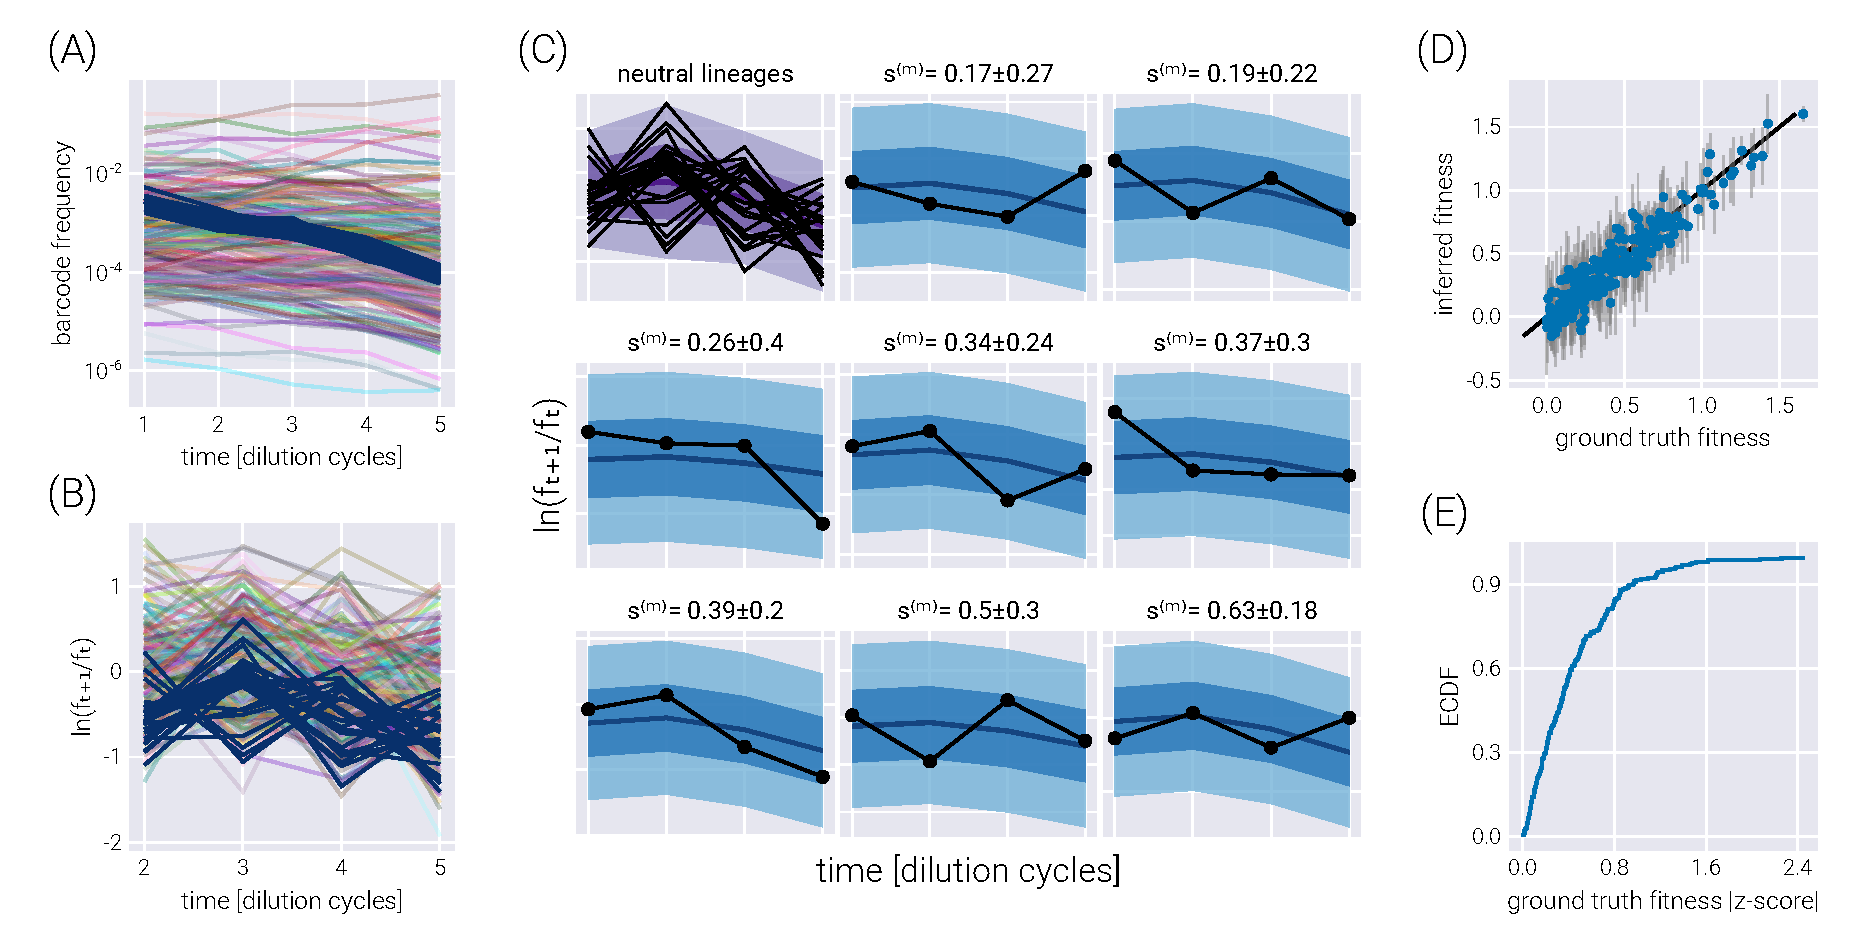
\includegraphics{./figs/fig02.pdf}

}

\caption{\label{fig-02}\textbf{Single dataset inference}. (A) Frequency
trajectories that represent the raw data going into the inference. (B)
Log frequency ratio between two adjacent time points used by the
inference pipeline. Darker lines represent the neutral barcodes. These
transformed data are much more noisy than the seemingly smooth frequency
trajectories. (C) Examples of the posterior predictive checks for all
neutral lineages (upper left panel) and a subset of representative
mutant lineages. Shaded regions represent the 95\%, 68\%, and 5\%
credible regions for the data. The reported errors above the plot
represent the 68\% credible region on the mutant relative fitness
marginal distribution. (D) Comparison between the ground truth fitness
value from the logistic-growth simulation and the inferred fitness
value. Gray error bars represent the 68\% posterior credible region for
the relative fitness values. (E) The empirical cumulative distribution
function (ECDF) for the absolute z-score value of the ground truth
parameter value within the inferred fitness posterior distribution.}

\end{figure}

\hypertarget{sec-multienv}{%
\subsection{Fitness inference on multiple
environments}\label{sec-multienv}}

The fitness model in Equation~\ref{eq-fitness} relates nuisance
parameters such as the population mean fitness and the barcode
frequencies to the relative fitness parameter we want to infer from the
data. These dependencies imply that uncertainty on the estimates of
these nuisance parameters influences the inference of the relevant
parameters. For example, imagine a scenario where the neutral lineages
data were incredibly noisy, leading to poor estimates of the population
mean fitness values \(\underline{\bar{s}}_T\). Since the relative
fitness of any non-neutral barcode \(s^{(m)}\) is determined with
respect to these neutral barcodes, not accounting for the lack of
precision in the value of the population mean fitness would result in
misleading estimates of the accuracy with which we determine the value
of the parameter we care about. Thus, propagating these sources of
uncertainty in nuisance parameters is vital to generate an unbiased
estimate of the relevant information we want to extract from the data.
One of the benefits of Bayesian methods is the intrinsic error
propagation embedded in the mathematical framework. For our previous
example, the uncertainty on the value of the population mean fitness
values is propagated to the relative fitness of a non-neutral barcode
since we defined a joint posterior distribution over all parameters as
fully expressed in Equation~\ref{eq-bayes_full}.

This natural error propagation can help us with the experimental design
schematized in Figure~\ref{fig-03}(A). Here, rather than performing
growth-dilution cycles in the same environment, the cells are diluted
into a different environment. Thus, the uncertainty on the fitness
estimate for the previous environment must be propagated to that of the
next one. To validate the extension of our statistical model to this
scenario, Figure~\ref{fig-03}(B) shows the trajectory of the log
frequency ratios between adjacent time points. The different colored
regions correspond to the different environments. For this simulation,
the growth rate of Environment 2 was set to be, on average, half of the
average growth rate in Environment 1. Equivalently, the growth rate in
Environment 3 was set to be, on average, twice the average growth rate
in Environment 1. Figure~\ref{fig-03}(C-E) show the correspondence
between the simulation ground truth and the inferred fitness values,
where the error bars represent the 68\% credible region.
Figure~\ref{fig-03}(F) summarizes the performance of our inference
pipeline by showing the empirical cumulative distribution functions for
the absolute value of the ground truth fitness value z-score within the
posterior distribution. This plot shows that, overall, \(\approx 75\%\)
of inferred mean values fall within one standard deviation of the ground
truth. For completeness, Figure~\ref{fig-03}(G) shows the posterior
predictive checks for a few example barcodes.

\begin{figure}

{\centering 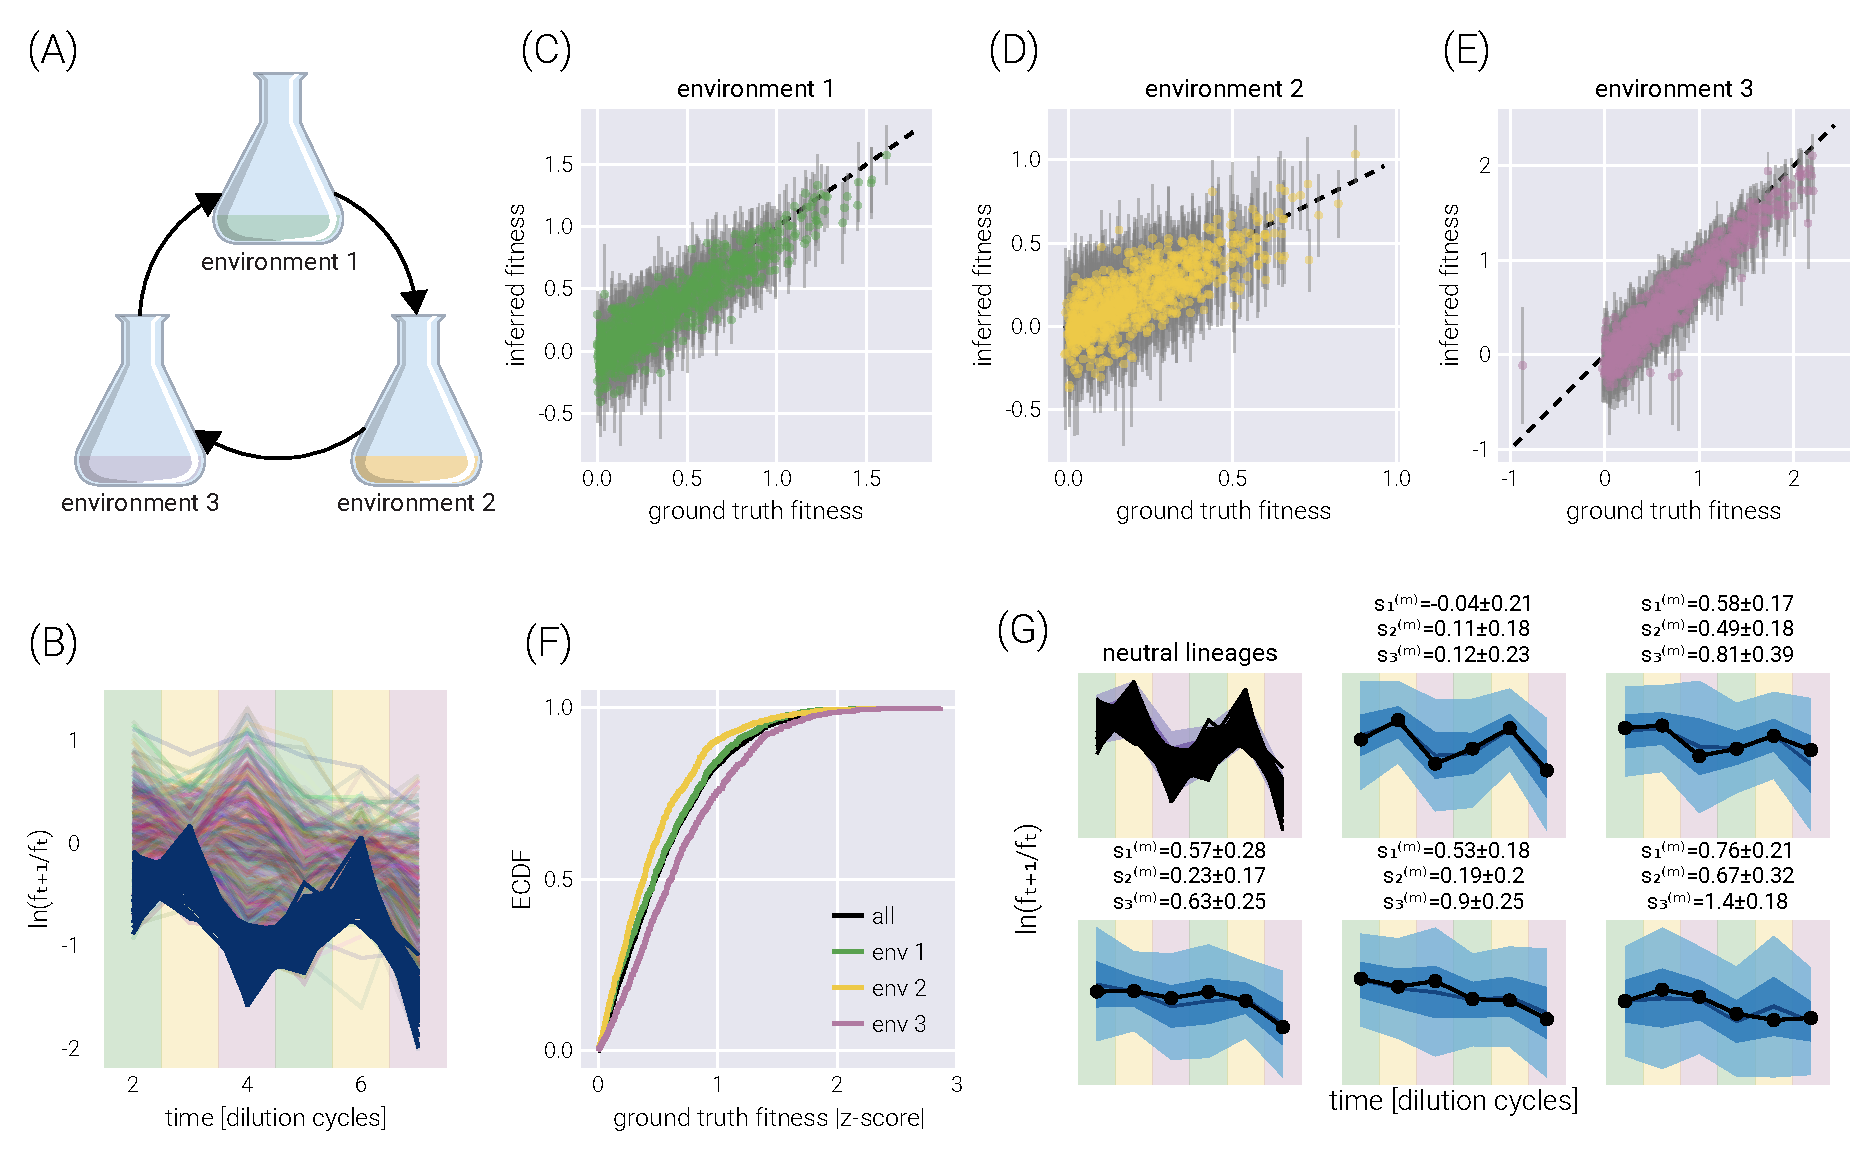
\includegraphics{./figs/fig03.pdf}

}

\caption{\label{fig-03}\textbf{Multi-environment fitness inference.} (A)
Schematic of the simulated experimental design where growth-dilution
cycles are performed into different environments for each cycle. (B) log
frequency rations between adjacent time points. Darker lines represent
the neutral barcodes. The colors in the background demark the
corresponding environment, matching colors in (A). Environment 2 is set
to have, on average, half the growth rate of environment 1. Likewise,
environment 3 is set to have, on average, twice the growth rate of
environment 1. (C-E) Comparison between the ground truth fitness value
from the logistic-growth simulation and the inferred fitness value for
each environment. Gray error bars represent the 68\% posterior credible
region. (F) The empirical cumulative distribution function (ECDF) for
the absolute z-score value of the ground truth parameter value within
the inferred fitness posterior distribution for all fitness values
(black line) and each environment individually (color lines). (G)
Examples of the posterior predictive checks for all neutral lineages
(upper left panel) and a subset of representative mutant lineages.
Shaded regions surrounding the data represent the 95\%, 68\%, and 5\%
credible regions for the data. The reported errors above the plot
represent the 68\% credible region on the mutant relative fitness
marginal distribution. Background colors match those of (A).}

\end{figure}

\hypertarget{sec-replicates}{%
\subsection{Accounting for experimental replicates via hierarchical
models}\label{sec-replicates}}

Our inference pipeline can be extended to account for multiple
experimental replicates via Bayesian hierarchical models
\autocite{betancourt2013}. Briefly, when accounting for multiple
repeated measurements of the same phenomena, there are two extreme cases
one can use to perform the data analysis: On the one hand, we can treat
each measurement as entirely independent, losing the power to utilize
multiple measurements when trying to learn a single parameter. This can
negatively impact the inference since, in principle, the value of our
parameter of interest should not depend on the particular experimental
replicate in question. However, this approach does not allow us to
properly ``combine'' the uncertainties in both experiments when
performing the inference. On the other hand, we can pool all data
together and treat our different experiments as a single measurement
with higher coverage. This loses the subtle differences due to biotic
and abiotic batch effects, effectively halving the data that goes into
our inference problem.

Hierarchical models present a middle ground between these extremes.
First, hierarchical models rely on the definition of so-called
\emph{hyper-parameters}, that capture the parametric inference we are
interested in---for this inference problem, we have a hyper-fitness
value \(\theta^{(m)}\) for each non-neutral barcode. Second, each
experiment draws randomly from the distribution of this hyper-parameter,
allowing for subtle variability between experiments to be accounted
for---in the present inference pipeline, each experimental replicate
gets assigned a \emph{local} fitness value \(s^{(m)}_i\), where the
extra sub-index indicates the \(i\)-th experimental replicate.
Conceptually, we can think of the local fitness for replicate \(i\) as
being sampled from a distribution that depends on the value of the
global hyper-fitness value, i.e., \(s^{(m)}_i \sim \pi_{\theta^{(m)}}\),
where the subindex \(\theta^{(m)}\) indicates the distribution's
parametric dependence on the hyper-fitness value. This way of
interpreting the connection between the distribution
\(\pi_{\theta^{(m)}}\) and the local fitness implies that a large
replicate-to-replicate variability would lead to a broad hyper-fitness
distribution---implying a large uncertainty when determining the
parameter that characterizes the overall relative fitness. We point the
reader to Section~\ref{sec-hierarchical_model} for the full definition
of the hierarchical model used in this section. Importantly, as
schematized in Figure~\ref{fig-04}(A), the influence between different
experimental replicates runs both ways. First, the data from one
experimental replicate (\(\underline{\underline{R}}^M_k\) in the
diagram) informs all local fitness values via the global hyper-fitness
(upper panel in Figure~\ref{fig-04}(A)). Second, the local fitness value
is informed by the data from all experimental replicates via the same
global hyper-fitness parameter (lower panel in Figure~\ref{fig-04}(A)).

To test the performance of this model, we simulated two experimental
replicates with 1000 unique barcodes (see Figure~\ref{fig-04}(B-C))
where we randomly sampled a ground truth hyper-fitness value
\(\theta^{(m)}\) for each barcode. We sampled a variation from this
hyper-fitness value for each experimental replicate \(s^{(m)}_i\) to
capture experimental batch effects. Figure~\ref{fig-04}(D) shows the
relationship between hyper-fitness and replicate fitness values for this
simulation. The spread around the identity line represents the expected
batch-to-batch variation. The posterior predictive checks examples in
Figure~\ref{fig-04}(E) show that the hierarchical model can correctly
fit the data for each experimental replicate. Furthermore,
Figure~\ref{fig-04}(F-G) show a high correlation between the ground
truth and the inferred fitness values. The empirical cumulative
distribution functions shown in Figure~\ref{fig-04}(H-I) reveal that for
\(\approx 75\%\) of the non-neutral barcodes, the ground truth
hyper-fitness values fall within one standard deviation from the mean
value in the posterior distributions.

\begin{figure}

{\centering 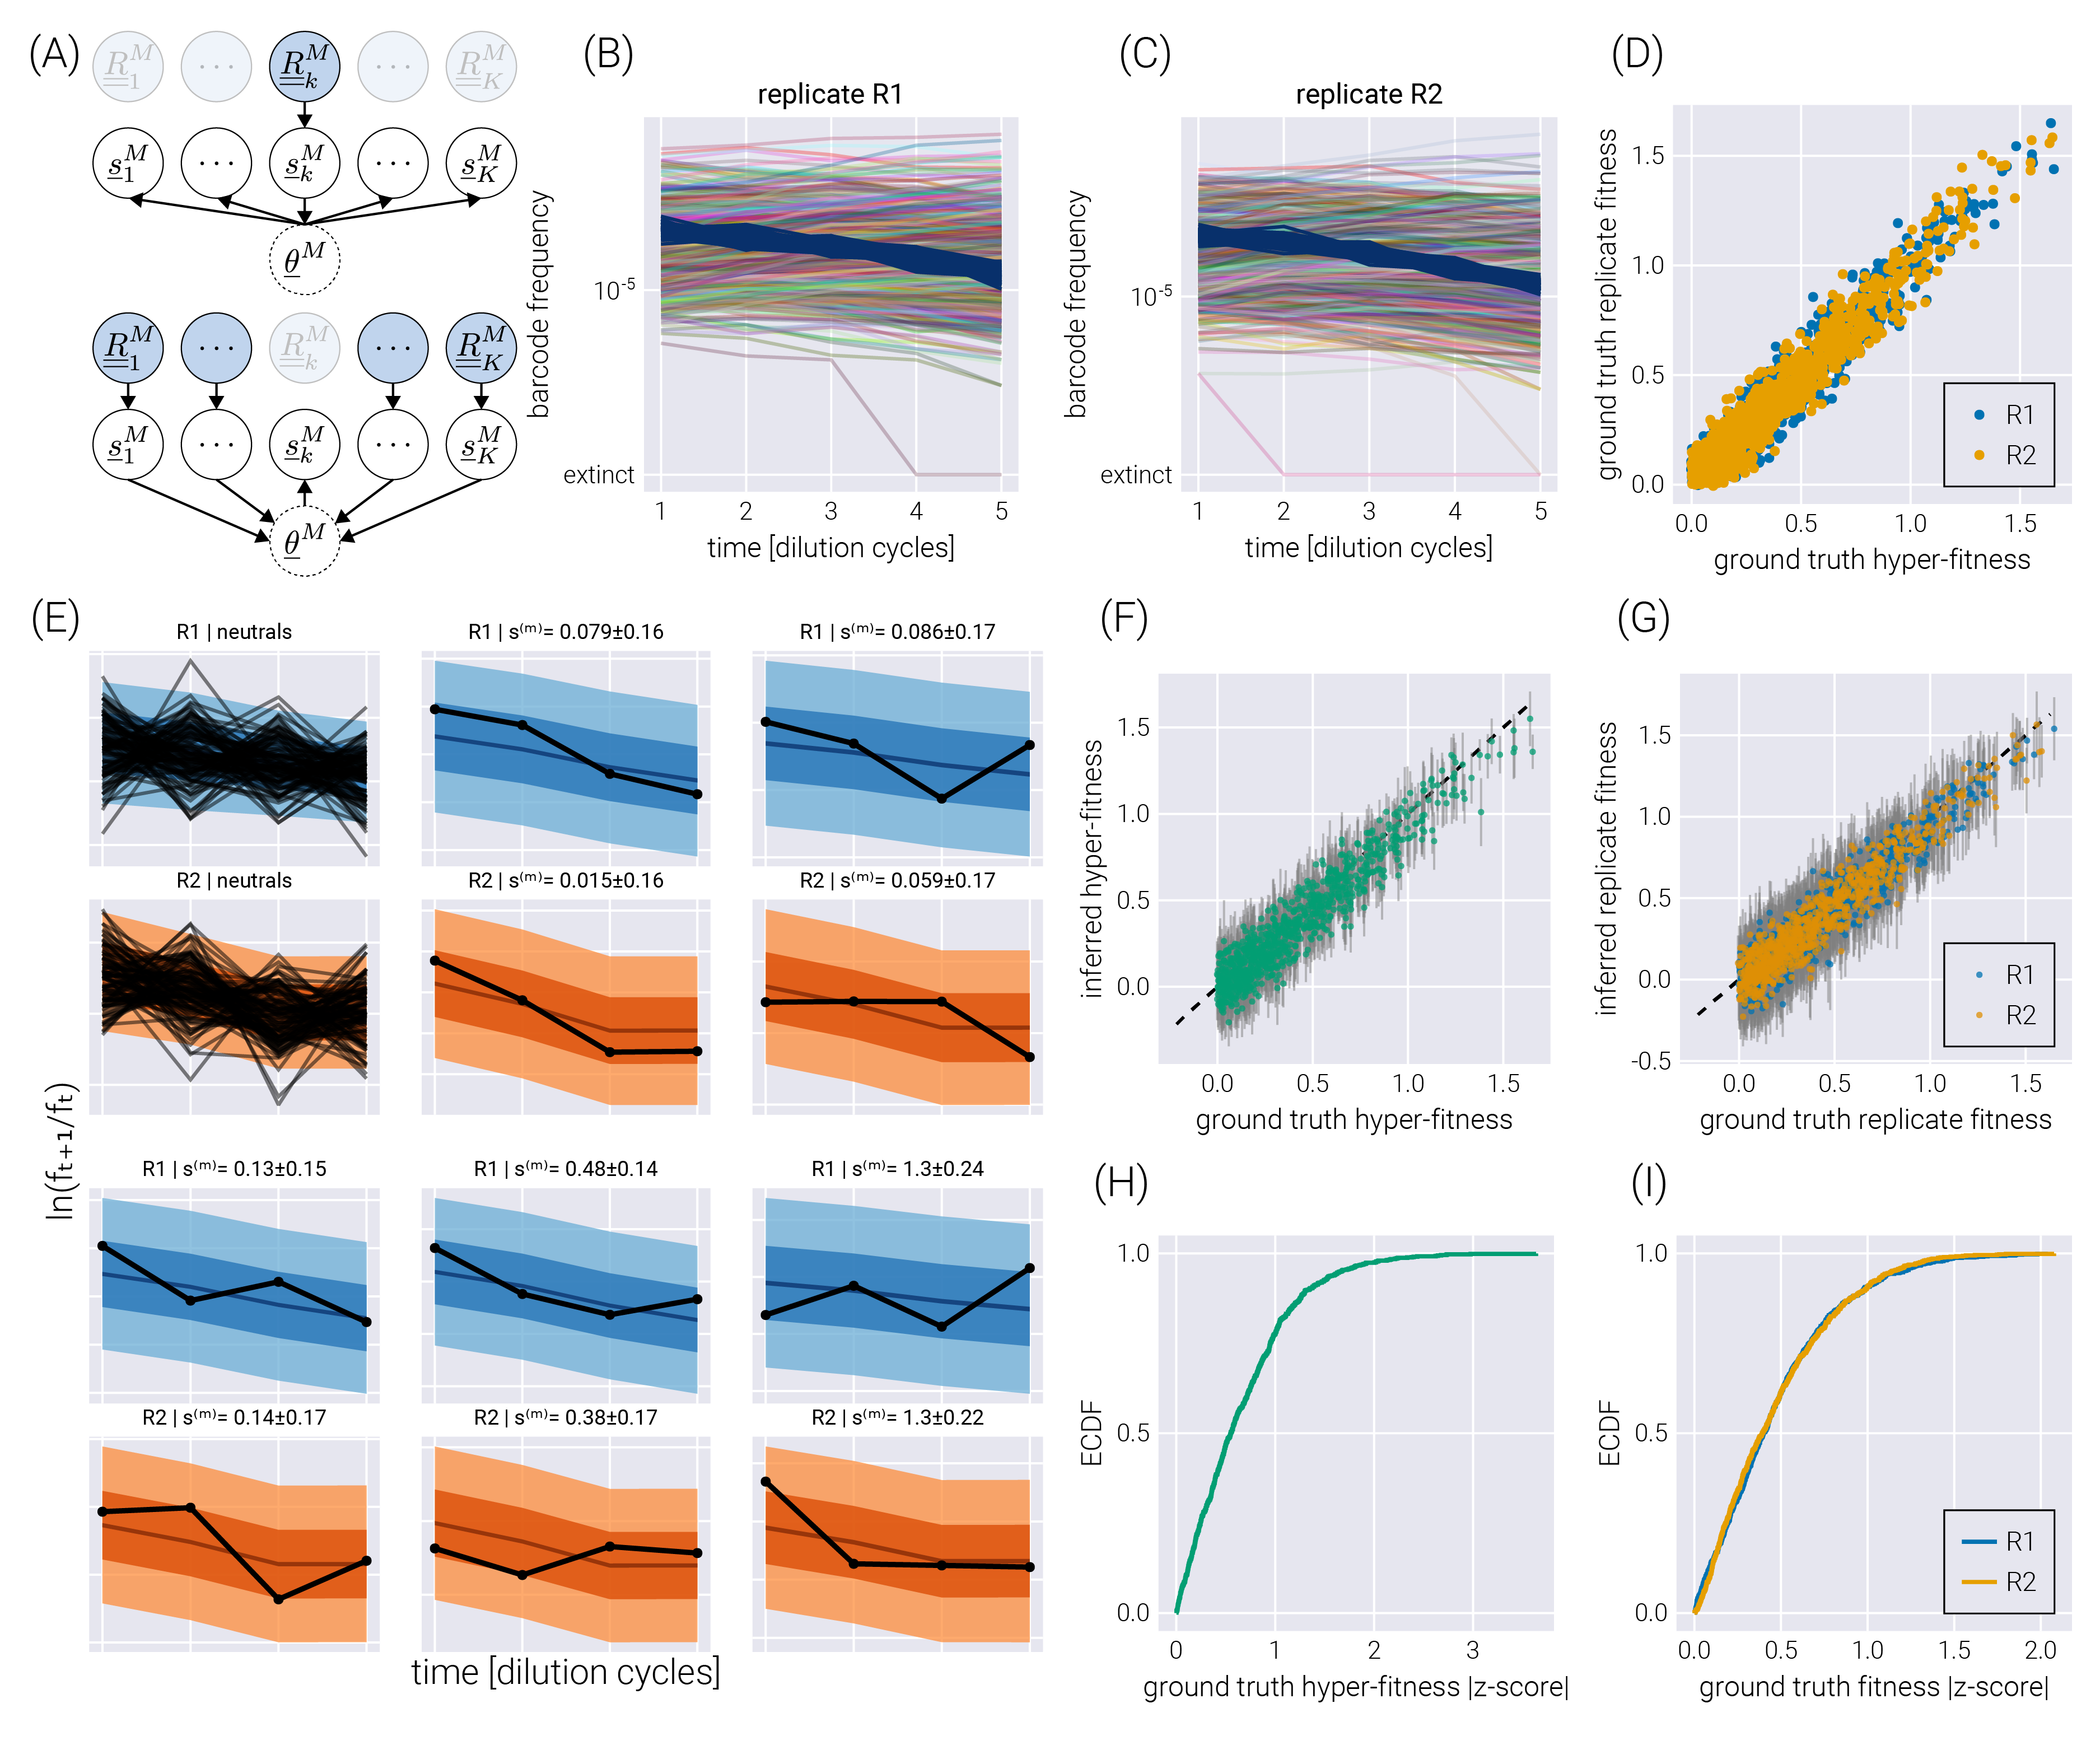
\includegraphics{./figs/fig04.pdf}

}

\caption{\label{fig-04}\textbf{Hierarchical model on experimental
replicates}. (A) Schematic depiction of the interactions between local
fitness values \(\underline{s}_k^M\) through the global hyper-fitness
value \(\underline{\theta}^M\) for \(K\) hypothetical experimental
replicates. The upper diagram shows how the data from replicate \(k\)
informs all local fitness values via the hyper-fitness parameter. The
lower panel shows the reverse, where all other datasets inform the local
fitness value. (B-C) Simulated replicate datasets with 900 barcodes of
interest and 100 neutral lineages. (D) Comparison between the simulation
ground truth hyper-fitness and each replicate ground truth fitness. The
scatter between parameters captures experimental batch effects. (E)
Examples of the posterior predictive checks for all neutral lineages
(upper left panels) and a subset of representative mutant lineages.
Shaded regions from light to dark represent the 95\%, 68\%, and 5\%
credible regions. (F-G) Comparison between the simulation's ground truth
hyper-fitness (F) and replicate fitness (G) values and the inferred
parameters. Gray error bars represent the 68\% posterior credible
region. (H-I) The empirical cumulative distribution function (ECDF) for
the absolute z-score value of the ground truth parameter value within
the inferred hyper-fitness posterior distribution (H) and replicate
fitness (I).}

\end{figure}

As shown in Figure~\ref{fig-05}, the structure imposed by the
hierarchical model schematized in Figure~\ref{fig-04}(A), where we
explicitly account for the connection between experimental replicates
can improve the quality of the inference. Inferred fitness values
between experimental replicates exhibit a stronger degree of correlation
in the hierarchical model (Figure~\ref{fig-05}(A)) compared to
conducting inference on each replicate independently
(Figure~\ref{fig-05}(B)). Moreover, when comparing the inferred
hyper-fitness values---the objective parameter when performing multiple
experimental measurements---the hierarchical model outperforms averaging
the independent experimental replicates as shown in
Figure~\ref{fig-05}(C) and (D).

\begin{figure}

{\centering 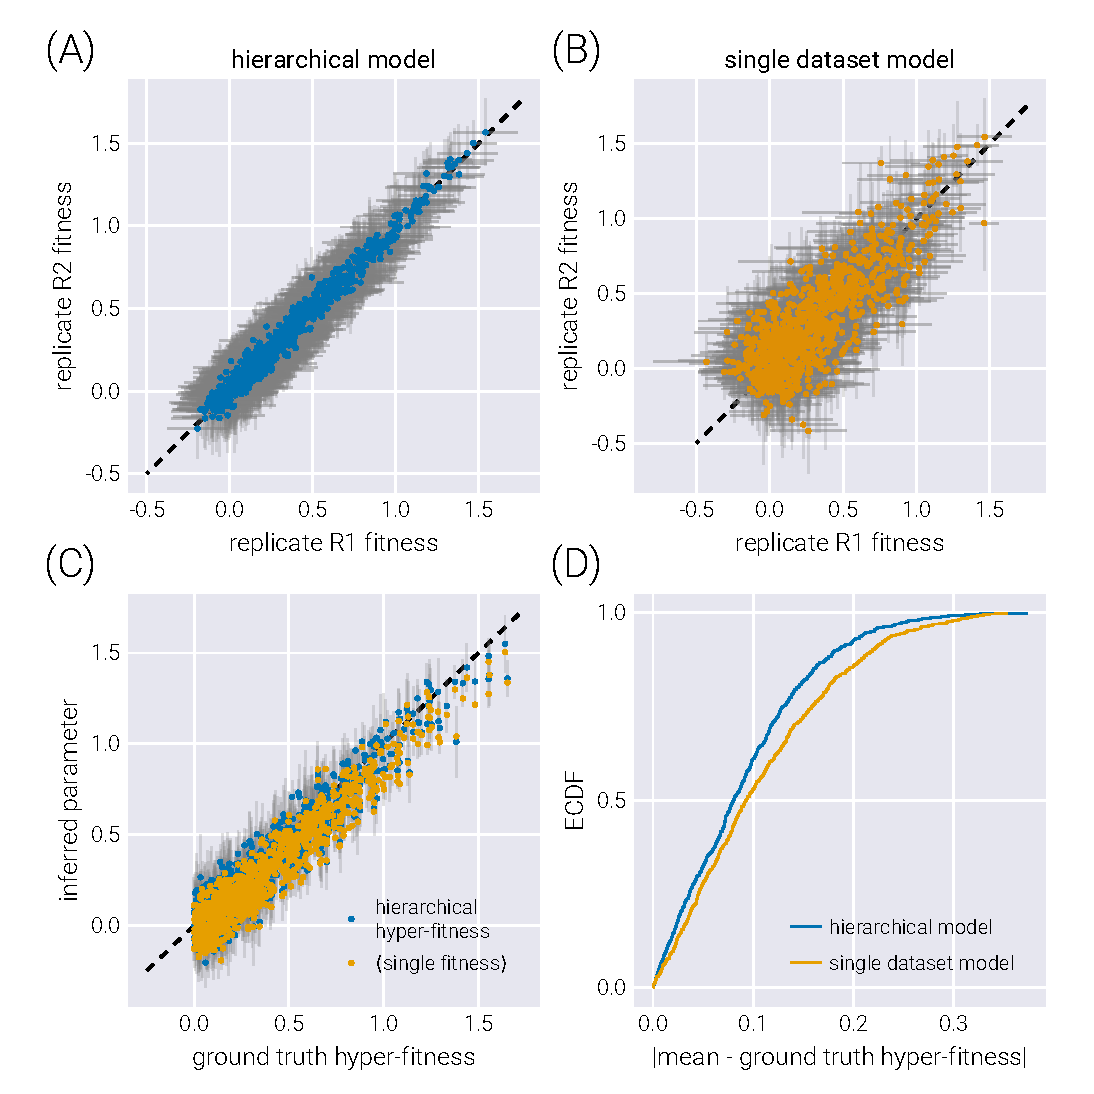
\includegraphics{./figs/fig05.pdf}

}

\caption{\label{fig-05}\textbf{Comparison between hierarchical model and
single dataset model}. (A-B) comparison of inferred fitness values
between experimental replicates when fitting a hierarchical model (A) or
independently fitting each dataset (B). Gray error bars represent the
68\% credible regions. (C) Comparison between the ground truth
hyper-fitness value and the inferred parameters. The blue dots show the
inferred hyper-fitness values when assuming a hierarchical model. Gray
error bars show the 68\% credible region for this inference. The yellow
dots show the average of the mean inferred fitness values for the two
experimental replicates. No error bars are shown for these, as it is
inappropriate to compute one with two data points per non-neutral
barcode. (D) Empirical cumulative distribution function (ECDF) of the
absolute difference between the inferred mean and the ground truth
hyper-fitness.}

\end{figure}

\hypertarget{sec-genotypes}{%
\subsection{Accounting for multiple barcodes per genotype via
hierarchical models}\label{sec-genotypes}}

Hierarchical models can also capture another experimental design in
which multiple barcodes map to the same or an equivalent genotype. As we
will show, this many-to-one mapping can improve the inference compared
to the extreme cases of inferring the fitness of each barcode
independently or pooling the data of all barcodes mapping to a single
genotype. As schematized in Figure~\ref{fig-06}(A), a small modification
of the base model allows us to map the structure of our original model
to that of a hierarchical model with a fitness hyperparameter vector
\(\underline{\theta}^G\), where \(G\) is the number of genotypes in the
dataset.

Figure~\ref{fig-06}(B) shows a single experimental replicate in which 90
genotypes were assigned a random number of barcodes (a multinomial
distribution with a mean of ten barcodes per genotype) for a total of
900 non-neutral barcodes. To assess the performance of the hierarchical
model proposed in Figure~\ref{fig-06}(A), we performed inference using
this hierarchical model, as well as the two extreme cases of ignoring
the connection between the barcodes belonging to the same
genotype---equivalent to performing inference using the model presented
in Figure~\ref{fig-02}(A) over the barcodes---or pooling the data of all
barcodes belonging to the same genotype into a single count---equivalent
to performing inference using the model presented in
Figure~\ref{fig-02}(A) over the pooled barcodes.
Figure~\ref{fig-06}(C-D) shows the comparison between the simulation
ground truth and the inferred values for these three cases. Not only do
the hierarchical model results show higher degrees of correlation with
the ground truth, but the error bars (representing the 68\% credible
regions) are smaller, meaning that the uncertainty in the estimate of
the parameter we care about decreases when using the hierarchical model.
The improvement in the prediction can be seen in Figure~\ref{fig-06}(F)
where the empirical cumulative distribution function of the absolute
difference between the mean inferred value and the simulation ground
truth is shown for all three inference models. The hierarchical model's
curve ascends more rapidly, showing that, in general, the inferred
values are closer to the ground truth. For completeness,
Figure~\ref{fig-06}(G) shows some examples of how the hierarchical model
can capture the raw log-frequency count observations.

\begin{figure}

{\centering 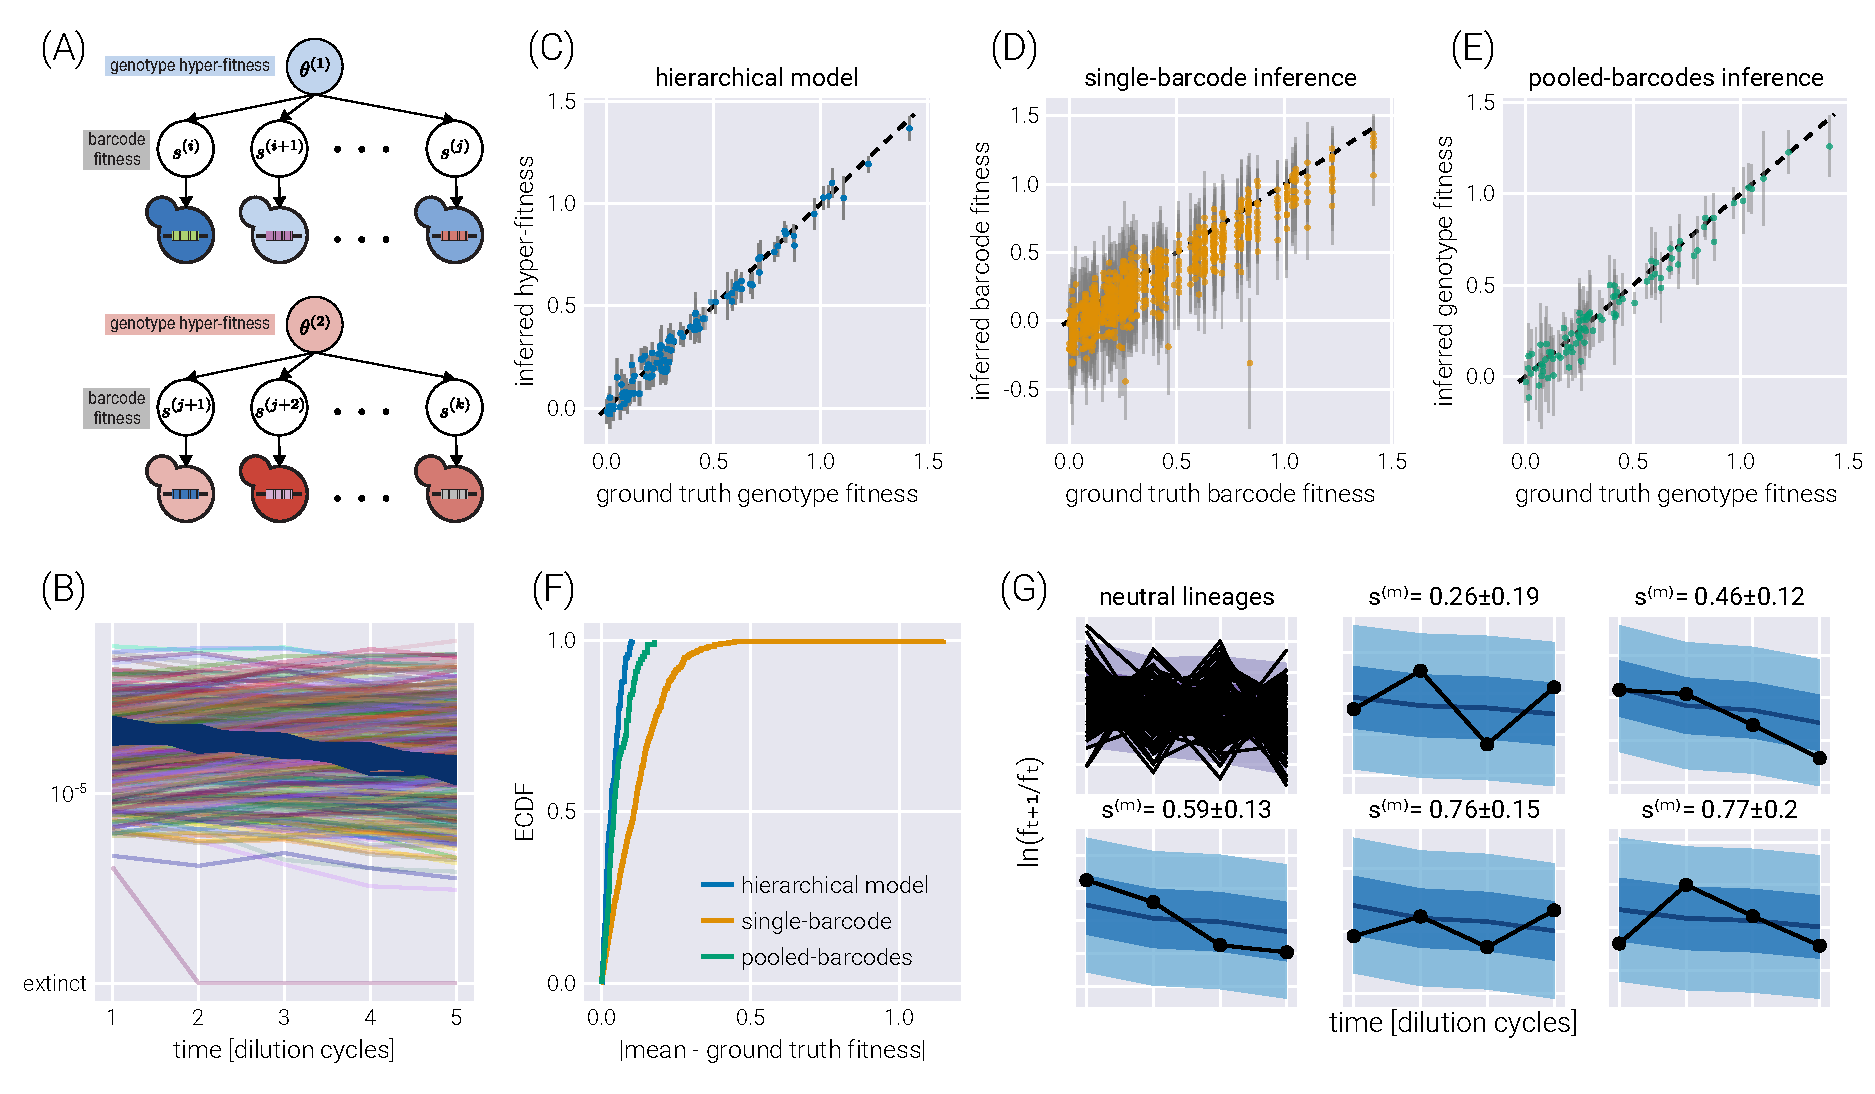
\includegraphics{./figs/fig06.pdf}

}

\caption{\label{fig-06}\textbf{Hierarchical model for multiple barcodes
per genotype.} (A) Schematic depiction of the hierarchical structure for
multiple barcodes mapping to a single genotype. A set of barcodes
mapping to an equivalent genotype map to ``local'' fitness values
\(s^{(b)}\) that are connected via a hyper-fitness parameter for the
genotype \(\theta^{(g)}\). (B) Simulated dataset with 100 neutral
lineages and 900 barcodes of interest distributed among 90 genotypes.
(C-E) Comparison between the inferred and ground truth fitness values
for a hierarchical model (C), a model where each barcode is inferred
independently (D), and a model where barcodes mapping to the same
genotype are pooled together (E). Gray error bars represent the 68\%
credible regions. (F) Empirical cumulative distribution function (ECDF)
of the absolute difference between the inferred mean and the ground
truth fitness values for all three models. (G) Examples of the posterior
predictive checks for all neutral lineages (upper left panels) and a
subset of representative mutant lineages. Shaded regions from light to
dark represent the 95\%, 68\%, and 5\% credible regions.}

\end{figure}

\hypertarget{discussion}{%
\section{Discussion}\label{discussion}}

Experimental evolution of microbial systems has dramatically advanced
our understanding of the basic principles of biological evolution
\autocite{kussell2013}. From questions related to the optimal
fine-tuning of gene expression programs \autocite{Dekel2005}, to the
dimensionality, geometry, and accessibility of the adaptive fitness
landscape explored by these rapidly adapting populations
\autocite{kinsler2020,maeda2020}, to the emergence of eco-evolutionary
dynamics in a long-term evolution experiment \autocite{good2017}; for
all of these and other cases, the microbial experimental platform
combined with high-throughput sequencing has been essential to tackling
these questions with empirical data. This exciting research area
promises to improve as new culturing technologies \autocite{jagdish2022}
as well as more complex lineage barcoding schemes
\autocite{nguyenba2019a,yang2022}, are adopted.

For this data-heavy field, properly accounting for the uncertainty in
parameters inferred from experiments is vital to ensure the conclusions
drawn are reliable. Bayesian statistics presents a principled way to
quantify this uncertainty systematically \autocite{gelman2010}.
Moreover, Bayesian analysis offers a more natural way to interpret the
role that probability theory plays when performing data analysis
compared to the often-misinterpreted frequentist methods
\autocite{vanderplas2014}. Nevertheless, the technical challenges
associated with Bayesian analysis has limited its application. This is
set to change as recognition of the misuse of frequentist concepts such
as the p-value is receiving more attention \autocite{nuzzo2014}.
Moreover, advances in numerical methods such as Hamiltonian Monte Carlo
\autocite{betancourt2017} and variational inference
\autocite{kucukelbir2016} allows for complex Bayesian models to be fit
to empirical data.

In this paper, we present a computational pipeline to analyze
lineage-tracking time-series data for massive-parallel competition
assays. More specifically, we fit a Bayesian model to infer the fitness
of multiple genotypes relative to a reference
\autocite{kinsler2020,ascensao2023}. The proposed model accounts for
multiple sources of uncertainty with proper error propagation intrinsic
to Bayesian methods. To scale the inference pipeline to large datasets
with \(> 10,000\) barcodes, we use the ADVI algorithm
\autocite{kucukelbir2016} to fit a variational posterior distribution.
The main difference between our method and previous inference pipelines,
such as \textcite{li2023}, is that the present analysis provides
interpretable errors on the inferred fitness values. The reported
uncertainty intervals---known as credible regions---can be formally
interpreted as capturing the corresponding probability mass of finding
the true value of the parameter given the model, the prior information,
and the data. Furthermore, minor modifications to the structure of the
statistical model presented in this work allow for the analysis of
different experimental designs, such as growth-dilution cycles in
different environments, joint analysis of multiple experimental
replicates of the same experiment via hierarchical models, and a
hierarchical model for multiple barcodes mapping to equivalent
genotypes. We validate our analysis pipeline on simulated datasets with
known ground truth, showing that the model fits the data adequately,
capturing the ground truth parameters within the posterior distribution.

It is important to highlight some of the consequences of the general
experimental design and the implicit assumptions within the proposed
statistical model to analyze the resulting data. First, the composition
of the population is such that the initial fraction of the population
occupied by the barcoded genotypes is small---usually \textgreater90\%
of the initial population is the non-labeled reference strain. This
constraint is important as the fitness model used to fit the time series
data assumes that the tracked frequencies are \(\ll 1\). Second, when
computing log frequency ratios, we can run into the issue of dividing by
zero. This is a common problem when dealing with molecular count data
\autocite{lovell2020}. Our model gets around this issue by assuming that
the frequency of any barcode cannot be, but still can get arbitrarily
close to, zero. Therefore, we implicitly assume that no lineage goes
extinct during the experiment. Moreover, the statistical model directly
accounts for the uncertainty associated with having zero barcode counts,
increasing the corresponding uncertainty. Third, the models presented in
this paper require the existence of a labeled sub-population of barcoded
reference strains. These barcodes help determine the fitness baseline,
as every fitness is quantified with respect to this reference genotype.
This experimental design constraint facilitates the inference of the
population mean fitness since most of the culture---the unlabeled
reference genotype---is not tracked. Finally, the presented statistical
model assumes that relative fitness is solely a constant of the
environment and the genotype. Future directions of this work could
extend the fitness model to properly analyze data with time-varying or
frequency-dependent fitness values.

In total, the statistical model presented in this work and the software
package accompanying the paper allow for a principled way of quantifying
the accuracy with which we can extract relevant parametric information
from large-scale multiplexed fitness competition assays. Furthermore,
the implementation of Bayesian models and their fitting via automatic
differentiation approaches opens the gate to extend this type of formal
analysis to the data-rich literature in experimental evolution and other
high-throughput technologies applications.

\hypertarget{acknowledgements}{%
\section{Acknowledgements}\label{acknowledgements}}

We would like to thank Griffin Chure and Michael Betancourt for their helpful
advice and discussion. We would like to thank Karna Gowda, Spencer Farrell, and
Shaili Mathur for critical observations on the manuscript. MRM was supported by
the Schmidt Science Fellowship. MM was supported by The National Science
Foundation-Simons Center for Quantitative Biology at Northwestern University and
the Simons Foundation grant 597491. MM is a Simons Investigator.

% Print main text references
\printbibliography[segment=\therefsegment]
% Close reference segment
\end{refsegment}

\clearpage

% SUPPLEMENTAL MATERIAL

% Indicate that now all sections and subsections should be included in the
% table of contents so that only the SI is included.
\addtocontents{toc}{\protect\setcounter{tocdepth}{3}}

% Define reference section for the supplemental material
\begin{refsegment}
% Set equation, table and figure counters to begin with "S"
\beginsupplement

\hypertarget{supplementary-materials}{%
\section{Supplementary Materials}\label{supplementary-materials}}

\tableofcontents

\hypertarget{sec-vi_primer}{%
\subsection{Primer on Variational Inference}\label{sec-vi_primer}}

In this section, we will briefly introduce the idea behind variational
inference. Recall that any Bayesian inference problem deals with the
joint distribution between observations \(\underline{x}\) and unobserved
latent variables \(\underline{\theta}\). This joint distribution can be
written as the product of a distribution of the observations
\(\underline{x}\) conditioned on the \(\underline{\theta}\) and the
marginal distribution of these latent variables, i.e.,
\begin{equation}\protect\hypertarget{eq-vi_joint_dist}{}{
\pi(\underline{x}, \underline{\theta}) =
\pi(\underline{x} \mid \underline{\theta}) \pi(\underline{\theta}).
}\label{eq-vi_joint_dist}\end{equation} A Bayesian inference pipeline's
objective is to compute the latent variables' posterior probability
given a set of observations. This computation is equivalent to updating
our prior beliefs about the set of values that the latent variables take
after taking in new data. We write this as Bayes theorem
\begin{equation}\protect\hypertarget{eq-vi_bayes_theorem}{}{
\pi(\underline{\theta} \mid \underline{x}) = 
\frac{
        \pi(\underline{x} \mid \underline{\theta})\pi(\underline{\theta})
    }{
        \pi(\underline{x})
    }.
}\label{eq-vi_bayes_theorem}\end{equation} The main technical challenge
for working with Equation~\ref{eq-vi_bayes_theorem} comes from the
computation of the denominator, also known as the \emph{evidence} or the
\emph{marginalized likelihood}. The reason computing this term is
challenging is because it involves a (potentially) high-dimensional
integral of the form
\begin{equation}\protect\hypertarget{eq-vi_evidence_int}{}{
\pi(\underline{x}) = 
\int\cdots\int d^K\underline{\theta}\; \pi(\underline{x}, \underline{\theta}) = 
\int\cdots\int d^K\underline{\theta}\; 
\pi(\underline{x} \mid \underline{\theta})
\pi(\underline{\theta}),
}\label{eq-vi_evidence_int}\end{equation} where \(K\) is the
dimesionality of the \(\underline{\theta}\) vector. Here, the integrals
are taken over the support---the set of values valid for the
distribution---of \(\pi(\underline{\theta})\). However, only a few
selected distributions have a closed analytical form; thus, in most
cases Equation~\ref{eq-vi_evidence_int} must be solved numerically.

Integration in high-dimensional spaces can be computationally extremely
challenging. For a naive numerical quadrature procedure, integrating
over a grid of values for each dimension of \(\underline{\theta}\) comes
with an exponential explosion of the number of required grid point
evaluations, most of which do not contribute significantly to the
integration. To gain visual intuition about this challenge, imagine
integrating the function depicted in Figure~\ref{fig-SI01}. If the
location of the high-density region (dark peak) is unknown, numerical
quadrature requires many grid points to ensure we capture this peak.
However, most of the numerical evaluations of the function on the grid
points do not contribute significantly to the integral. Therefore, our
computational resources are wasted on insignificant evaluations. This
only gets worse as the number of dimensions increases since the number
of grid point evaluation scales exponentially.

\begin{figure}

{\centering 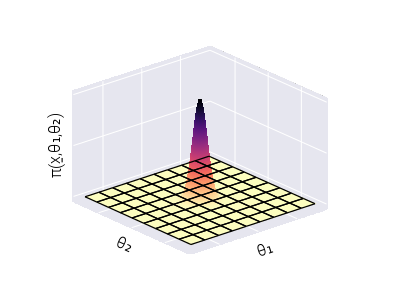
\includegraphics{./figs/figSIX_gaussian_peak.png}

}

\caption{\label{fig-SI01}\textbf{High-dimensional numerical quadrature
does not scale with dimensionality.} Schematic depiction of the problem
with naive numerical quadrature to integrate over an unknown density.
While the density is concentrated on the dark peak, most of the
evaluations over the \(x_1-x_2\) grid do not contribute to the value of
the integral}

\end{figure}

Modern Markov Chain Monte Carlo algorithms, such as Hamiltonian Monte
Carlo, can efficiently perform this high-dimensional integration by
utilizing gradient information from the target density
\textcite{betancourt2017}. Nevertheless, these sampling-based methods
become prohibitively slow for the number of dimensions our present
inference problem presents. Thus, there is a need to find scalable
methods for the inference problem in Equation~\ref{eq-vi_bayes_theorem}.

Variational inference circumvents these technical challenges by
proposing an approximate solution to the problem. Instead of working
with the posterior distribution in its full glory
\(\pi(\underline{\theta} \mid \underline{x})\), let us propose an
approximate posterior distribution \(q_\phi\) that belongs to a
distribution family fully parametrized by \(\phi\). For example, let us
say that the distribution \(q_\phi\) belongs to the family of
multivariate Normal distributions such that
\(\phi = (\underline{\mu}, \underline{\underline{\Sigma}})\), where
\(\underline{\mu}\) is the vector of means and
\(\underline{\underline{\Sigma}}\) is the covariance matrix. If we
replace \(\pi\) by \(q_\phi\), we want \(q_\phi\) to resemble the
original posterior as much as possible. Mathematically, this can be
expressed as minimizing a ``\emph{distance metric}''---the
Kullback-Leibler (KL) divergence, for example---between the
distributions. Note that we use quotation marks because, formally, the
KL divergence is not a distance metric since it is not symmetric.
Nevertheless, the variational objective is set to find a distribution
\(q_\phi^*\) such that
\begin{equation}\protect\hypertarget{eq-vi_objective}{}{
q_\phi^*(\underline{\theta}) =
\min_\phi D_{KL}\left(
    q_\phi(\underline{\theta}) \vert\vert 
    \pi(\underline{\theta} \mid \underline{x})
\right),
}\label{eq-vi_objective}\end{equation} where \(D_{KL}\) is the KL
divergence. Furthermore, we highlight that the KL divergence is a
strictly positive number, i.e.,
\begin{equation}\protect\hypertarget{eq-vi_kl_pos}{}{
D_{KL}\left(
    q_\phi(\underline{\theta}) \vert\vert 
    \pi(\underline{\theta} \mid \underline{x})
\right) \geq 0,
}\label{eq-vi_kl_pos}\end{equation} as this property will become
important later on.

At first sight, Equation~\ref{eq-vi_objective} does not improve the
situation but only introduces further technical complications. After
all, the definition of the KL divergence
\begin{equation}\protect\hypertarget{eq-vi_kl_div}{}{
D_{KL}\left(
    q_\phi(\underline{\theta}) \vert\vert 
    \pi(\underline{\theta} \mid \underline{x})
\right) \equiv 
\int \cdots \int d^K\underline{\theta}\;
q_\phi(\underline{\theta})
\ln \frac{
    q_\phi(\underline{\theta})
}{
    \pi(\underline{\theta} \mid \underline{x})
},
}\label{eq-vi_kl_div}\end{equation} includes the posterior distribution
\(\pi(\underline{\theta} \mid \underline{x})\) we are trying to get
around. However, let us manipulate Equation~\ref{eq-vi_kl_div} to beat
it to a more reasonable form. First, we can use the properties of the
logarithms to write
\begin{equation}\protect\hypertarget{eq-vi_step01}{}{
D_{KL}\left(
    q_\phi(\underline{\theta}) \vert\vert 
    \pi(\underline{\theta} \mid \underline{x})
\right) = 
\int d^K\underline{\theta}\; q_\phi(\underline{\theta})
\ln q_\phi(\underline{\theta}) -
\int d^K\underline{\theta}\; q_\phi(\underline{\theta})
\ln \pi(\underline{\theta} \mid \underline{x}),
}\label{eq-vi_step01}\end{equation} where, for convenience, we write a
single integration sign (\(d^K\underline{\theta}\;\) still represents a
multi-dimensional differential). For the second term in
Equation~\ref{eq-vi_step01}, we can substitute the term inside the
logarithm using Equation~\ref{eq-vi_bayes_theorem}. This results in
\begin{equation}\protect\hypertarget{eq-vi_step02}{}{
\begin{aligned}
D_{KL}\left(
    q_\phi(\underline{\theta}) \vert\vert 
    \pi(\underline{\theta} \mid \underline{x})
\right) &= 
\int d^K\underline{\theta}\; q_\phi(\underline{\theta})
\ln q_\phi(\underline{\theta}) \\
&- \int d^K\underline{\theta}\; q_\phi(\underline{\theta})
\ln \left( 
    \frac{
        \pi(\underline{x} \mid \underline{\theta})\pi(\underline{\theta})
    }{
        \pi(\underline{x})
    }
\right).
\end{aligned}
}\label{eq-vi_step02}\end{equation} Again, using the properties of
logarithms, we can split Equation~\ref{eq-vi_step02}, obtaining
\begin{equation}\protect\hypertarget{eq-vi_step03}{}{
\begin{aligned}
D_{KL}\left(
    q_\phi(\underline{\theta}) \vert\vert 
    \pi(\underline{\theta} \mid \underline{x})
\right) &= 
\int d^K\underline{\theta}\; q_\phi(\underline{\theta})
\ln q_\phi(\underline{\theta}) \\
&-\int d^K\underline{\theta}\; q_\phi(\underline{\theta})
\ln \pi(\underline{x} \mid \underline{\theta}) \\
&-\int d^K\underline{\theta}\; q_\phi(\underline{\theta})
\ln \pi(\underline{\theta}) \\
&+\int d^K\underline{\theta}\; q_\phi(\underline{\theta})
\ln \pi(\underline{x}).
\end{aligned}
}\label{eq-vi_step03}\end{equation} It is convenient to write
Equation~\ref{eq-vi_step03} as
\begin{equation}\protect\hypertarget{eq-vi_step04}{}{
\begin{aligned}
D_{KL}\left(
    q_\phi(\underline{\theta}) \vert\vert 
    \pi(\underline{\theta} \mid \underline{x})
\right) &= 
\int d^K\underline{\theta}\; q_\phi(\underline{\theta})
\ln \frac{
    q_\phi(\underline{\theta})
    }{
        \pi(\underline{\theta})
    } \\
&-\int d^K\underline{\theta}\; q_\phi(\underline{\theta})
\ln \pi(\underline{x} \mid \underline{\theta}) \\
&+ \ln \pi(\underline{x}) 
\int d^K\underline{\theta}\; q_\phi(\underline{\theta}),
\end{aligned}
}\label{eq-vi_step04}\end{equation} where for the last term, we can take
\(\ln \pi(\underline{x})\) out of the integral since it does not depend
on \(\underline{\theta}\). Lastly, we utilize two properties:

\begin{enumerate}
\def\labelenumi{\arabic{enumi}.}
\tightlist
\item
  The proposed approximate distribution must be normalized, i.e.,
  \begin{equation}\protect\hypertarget{eq-vi_q_norm}{}{
  \int d^K\underline{\theta}\; q_\phi(\underline{\theta}) = 1.
  }\label{eq-vi_q_norm}\end{equation}
\item
  The law of the unconscious statistician (LOTUS) establishes that for
  any probability density function, it must be true that
  \begin{equation}\protect\hypertarget{eq-vi_lotus}{}{
  \int d^K\underline{\theta}\; q_\phi(\underline{\theta})
  f(\underline{\theta}) = \left\langle 
   f(\underline{\theta}) 
  \right\rangle_{q_\phi},
  }\label{eq-vi_lotus}\end{equation} where
  \(\left\langle\cdot\right\rangle_{q_\phi}\) is the expected value over
  the \(q_\phi\) distribution.
\end{enumerate}

Using these two properties, the positivity constraint on the KL
divergence in Equation~\ref{eq-vi_kl_pos}, and the definition of the KL
divergence in Equation~\ref{eq-vi_kl_div} we can rewrite
Equation~\ref{eq-vi_step04} as
\begin{equation}\protect\hypertarget{eq-vi_step05}{}{
D_{KL}\left( 
    q_\phi(\underline{\theta}) \vert \vert
    \pi(\underline{\theta}) 
\right) -
\left\langle
    \ln \pi(\underline{x} \mid \underline{\theta})
\right\rangle_{q_\phi}
\geq - \ln \pi(\underline{x}).
}\label{eq-vi_step05}\end{equation} Multiplying by a minus one, we have
the functional form of the so-called evidence lower bound (ELBO)
\textcite{kingma2014},
\begin{equation}\protect\hypertarget{eq-vi_elbo}{}{
\underbrace{
    \ln \pi(\underline{x})
}_{\text{log evidence}} \geq
\underbrace{
    \left\langle
        \ln \pi(\underline{x} \mid \underline{\theta})
    \right\rangle_{q_\phi} -
    D_{KL}\left( 
        q_\phi(\underline{\theta}) \vert \vert
        \pi(\underline{\theta}) 
    \right)
}_{\text{ELBO}}.
}\label{eq-vi_elbo}\end{equation}

Let us recapitulate where we are. We started by presenting the challenge
of working with Bayes' theorem, as it requires a high-dimensional
integral of the form in Equation~\ref{eq-vi_evidence_int}. As an
alternative, variational inference posits to approximate the posterior
distribution \(\pi(\underline{\theta} \mid \underline{x})\) with a
parametric distribution \(q_\phi(\underline{\theta})\). By minimizing
the KL divergence between these distributions, we arrive at the result
in Equation~\ref{eq-vi_elbo}, where the left-hand side---the log
marginalized likelihood or log evidence---we cannot compute for
technical/computational reasons. However, the right-hand side is
composed of things we can easily evaluate. We can easily evaluate the
log-likelihood \(\ln \pi(\underline{x} \mid \underline{\theta})\) and
the KL divergence between our proposed approximate distribution
\(q_\phi(\underline{\theta})\) and the prior distribution
\(\pi(\underline{\theta})\). Moreover, we can compute the gradients of
these functions with respect to the parameters of our proposed
distribution. This last point implies that we can change the parameters
of the proposed distribution to maximize the ELBO. And, although we
cannot compute the left-hand side of Equation~\ref{eq-vi_elbo}, we know
that however large we make the ELBO, it will always be smaller than (or
equal) the log-marginal likelihood. Therefore, the larger we can make
the ELBO by modifying the parameters \(\phi\), the closer it gets to the
log-marginal likelihood, and, as a consequence, the better our proposed
distribution \(q_\phi(\underline{\theta})\) gets to the true posterior
distribution \(\pi(\underline{\theta} \mid \underline{x})\).

In this sense, variational inference turns the intractable numerical
integration problem to an optimization routine, for which there are
several algorithms available.

\hypertarget{advi-algorithm}{%
\subsubsection{ADVI algorithm}\label{advi-algorithm}}

To maximize the right-hand side of Equation~\ref{eq-vi_elbo}, the
Automatic Differentiation Variational Inference (ADVI) algorithm
developed in \autocite{kucukelbir2016} takes advantage of advances in
probabilistic programming languages to generate a robust method to
perform this optimization. Without going into the details of the
algorithm implementation, for our purposes, it suffices to say that we
define our joint distribution \(\pi(\underline{\theta}, \underline{x})\)
as the product defined in Equation~\ref{eq-vi_joint_dist}. ADVI then
proposes an approximate variational distribution \(q_\phi\) that can
either be a multivariate Normal distribution with a diagonal covariance
matrix, i.e., \begin{equation}\protect\hypertarget{eq-vi_meanfield}{}{
\phi = (\underline{\mu}, \underline{\underline{D}}),
}\label{eq-vi_meanfield}\end{equation} where
\(\underline{\underline{D}}\) is the identity matrix, with the diagonal
elements given by the vector of variances \(\underline{\sigma}^2\) for
each variable or a full-rank multivariate Normal distribution
\begin{equation}\protect\hypertarget{eq-vi_full}{}{
\phi = (\underline{\mu}, \underline{\underline{\Sigma}}).
}\label{eq-vi_full}\end{equation}

Then, the parameters are initialized in some value \(\phi_o\). These
parameters are iteratively updated by computing the gradient of the ELBO
(right-hand side of Equation~\ref{eq-vi_elbo}), hereafter defined as
\(\mathcal{L}\), with respect to the parameters,
\begin{equation}\protect\hypertarget{eq-vi_elbo_gradient}{}{
\nabla_\phi \mathcal{L} = \nabla_{\underline{\mu}} \mathcal{L} + 
\nabla_{\underline{\sigma}}\mathcal{L},
}\label{eq-vi_elbo_gradient}\end{equation} and then computing \[
\phi_{t+1} = \phi_{t} + \eta \nabla_\phi \mathcal{L},
\] where \(\eta\) defines the step size.

This short explanation behind the ADVI algorithm is intended only to
gain intuition on how the optimal variational distribution \(q_\phi\) be
computed. There are many nuances in the implementation of the ADVI
algorithm. We invite the reader to look at the original reference for
further details.

\hypertarget{sec-bayes_def}{%
\subsection{Defining the Bayesian model}\label{sec-bayes_def}}

In the main text, we specify the inference problem we must solve as
being of the form
\begin{equation}\protect\hypertarget{eq-full_inference_SI}{}{
\pi(
    \underline{s}^M, \underline{\bar{s}}_T, \underline{\underline{F}} \mid
    \underline{\underline{R}}
) \propto
\pi(
    \underline{\underline{R}} \mid
    \underline{s}^M, \underline{\bar{s}}_T, \underline{\underline{F}}
)
\pi(
    \underline{s}^M, \underline{\bar{s}}_T, \underline{\underline{F}}
).
}\label{eq-full_inference_SI}\end{equation} Here, we briefly define the
missing nuisance parameters. Let
\begin{equation}\protect\hypertarget{eq-pop_fitness_vec}{}{
\underline{\bar{s}}_T = (\bar{s}_1, \bar{s}_2, \ldots, \bar{s}_{T-1})^\dagger,
}\label{eq-pop_fitness_vec}\end{equation} be the vector containing the
\(T-1\) population mean fitness we compute from the \(T\) time points
where measurements were taken. We have \(T-1\) since the value of any
\(\bar{s}_t\) requires cycle numbers \(t\) and \(t+1\). Furthermore, let
the matrix \(\underline{\underline{F}}\) be a \(T \times B\) matrix
containing all frequency values. As with Equation~\ref{eq-R-mat_split}
in the main text, we can split \(\underline{\underline{F}}\) into two
matrices of the form
\begin{equation}\protect\hypertarget{eq-F-mat_split}{}{
\underline{\underline{F}} = \left[ 
\underline{\underline{F}}^N \; \underline{\underline{F}}^M
\right],
}\label{eq-F-mat_split}\end{equation} to separate the corresponding
neutral and non-neutral barcode frequencies.

Let us now define each of the terms in Equation~\ref{eq-split_posterior}
described in Section~\ref{sec-bayesian_inference} of the main text. The
following sections will specify the functional form each of these terms
takes.

\hypertarget{sec-bayes_freq}{%
\subsubsection{\texorpdfstring{Frequency uncertainty
\(\pi(\underline{\underline{F}} \mid \underline{\underline{R}})\)}{Frequency uncertainty \textbackslash pi(\textbackslash underline\{\textbackslash underline\{F\}\} \textbackslash mid \textbackslash underline\{\textbackslash underline\{R\}\})}}\label{sec-bayes_freq}}

We begin with the probability of the frequency values given the raw
barcode reads. The first assumption is that the inference of the
frequency values for time \(t\) is independent of any other time.
Therefore, we can write the joint probability distribution as a product
of independent distributions of the form
\begin{equation}\protect\hypertarget{eq-freq_indep}{}{
\pi(\underline{\underline{F}} \mid \underline{\underline{R}}) =
\prod_{t=1}^T \pi(\underline{f}_t \mid \underline{r}_t),
}\label{eq-freq_indep}\end{equation} where \(\underline{f}_t\) and
\(\underline{r}_t\) are the \(t\)-th row of the matrix containing all of
the measurements for time \(t\). We imagine that when the barcode reads
are obtained via sequencing, the quantified number of reads is a Poisson
sample from the ``true'' underlying number of barcodes within the pool.
This translates to assuming that the number of reads for each barcode at
any time point \(r^{(b)}_t\) is an independent Poisson random variable,
i.e., \begin{equation}\protect\hypertarget{eq-freq_poisson_reads}{}{
r^{(b)}_t \sim \operatorname{Poiss}(\lambda^{(b)}_t),
}\label{eq-freq_poisson_reads}\end{equation} where the symbol
``\(\sim\)'' is read ``distributed as.'' Furthermore, for a Poisson
distribution, we have that
\begin{equation}\protect\hypertarget{eq-freq_poisson_lambda}{}{
\lambda^{(b)}_t = \left\langle r^{(b)}_t \right\rangle = 
\left\langle 
    \left( r^{(b)}_t - \left\langle r^{(b)}_t \right\rangle \right)^2
\right\rangle,
}\label{eq-freq_poisson_lambda}\end{equation} where
\(\left\langle \cdot \right\rangle\) is the expected value. In other
words the Poisson parameter is equal to the mean and variance of the
distribution. The Poisson distribution has the convenient property that
for two Poisson distributed random variables
\(X \sim \operatorname{Poiss}(\lambda_x)\) and
\(Y \sim \operatorname{Poiss}(\lambda_y)\), we have that
\begin{equation}\protect\hypertarget{eq-freq_additivity}{}{
Z \equiv X + Y \sim \operatorname{Poiss}(\lambda_x + \lambda_y).
}\label{eq-freq_additivity}\end{equation} This additivity allows us to
write the total number of reads at time \(t\) \(n_t\) also as a
Poisson-distributed random variable of the form
\begin{equation}\protect\hypertarget{eq-freq_poisson_total}{}{
n_t \sim \operatorname{Poiss}\left( \sum_{b=1}^B \lambda^{(b)}_t \right),
}\label{eq-freq_poisson_total}\end{equation} where the sum is taken over
all \(B\) barcodes.

If the total number of reads is given by
Equation~\ref{eq-freq_poisson_total}, the array with the number of reads
for each barcode at time \(t\), \(\underline{r}_t\) is then distributed
as \begin{equation}\protect\hypertarget{eq-freq_multinomial}{}{
\underline{r}_t \sim \operatorname{Multinomial}(n_t, \underline{f}_t),
}\label{eq-freq_multinomial}\end{equation} where each of the \(B\)
entries of the frequency vector \(\underline{f}_t\) is a function of the
\(\underline{\lambda}_t\) vector, given by
\begin{equation}\protect\hypertarget{eq-freq_freq_lambda}{}{
f_t^{(b)} \equiv f_t^{(b)}(\underline{\lambda}_t) = 
\frac{\lambda_t^{(b)}}{\sum_{b'=1}^B \lambda_t^{(b')}}.
}\label{eq-freq_freq_lambda}\end{equation} In other words, we can think
of the \(B\) barcode counts as independent Poisson samples or as a
single multinomial draw with a random number of total draws, \(n_t\),
and the frequency vector \(\underline{f}_t\) we are interested in.
Notice that Equation~\ref{eq-freq_freq_lambda} is a deterministic
function that connects the Poisson parameters to the frequencies.
Therefore, we have the equivalence that
\begin{equation}\protect\hypertarget{eq-freq_f_lambda_equiv}{}{
\pi(\underline{f}_t \mid \underline{r}_t) = 
\pi(\underline{\lambda}_t \mid \underline{r}_t),
}\label{eq-freq_f_lambda_equiv}\end{equation} meaning that the
uncertainty comes from the \(\underline{\lambda}_t\) vector. By Bayes
theorem, we therefore write
\begin{equation}\protect\hypertarget{eq-freq_lambda_bayes}{}{
\pi(\underline{\lambda}_t \mid n_t, \underline{r}_t) \propto
\pi(n_t, \underline{r}_t \mid \underline{\lambda}_t) \pi(\underline{\lambda}_t),
}\label{eq-freq_lambda_bayes}\end{equation} where we explicitly include
the dependence on \(n_t\). This does not affect the distribution or
brings more uncertainty because \(\underline{r}_t\) already contains all
the information to compute \(n_t\) since
\begin{equation}\protect\hypertarget{eq-freq_n_sum_r}{}{
n_t = \sum_{b=1}^B r_t^{(b)}.
}\label{eq-freq_n_sum_r}\end{equation} But adding the variable allows us
to factorize Equation~\ref{eq-freq_lambda_bayes} as
\begin{equation}\protect\hypertarget{eq-freq_lambda_bayes_factorized}{}{
\pi(\underline{\lambda}_t \mid n_t, \underline{r}_t) \propto
\pi(\underline{r}_t \mid n_t, \underline{\lambda}_t)
\pi(n_t \mid \underline{\lambda}_t)
\pi(\underline{\lambda}_t)
}\label{eq-freq_lambda_bayes_factorized}\end{equation} We then have
\begin{equation}\protect\hypertarget{eq-freq_r_bayes}{}{
\underline{r}_t \mid n_t, \underline{\lambda}_t \sim
\operatorname{Multinomial}(n_t, \underline{f}_t(\underline{\lambda}_t)).
}\label{eq-freq_r_bayes}\end{equation} Furthermore, we have \[
n_t \mid \underline{\lambda}_t \sim 
\operatorname{Poiss}\left(\sum_{b=1}^B \lambda_t^{(b)}\right).
\]\{\#eq=freq\_n\_bayes\} Finally, for our prior
\(\pi(\underline{\lambda}_t)\), we first assume each parameter is
independent, i.e., \[
\pi(\underline{\lambda}_t) = \prod_{b=1}^B \pi(\lambda_t^{(b)}).
\] A reasonable prior for each \(\lambda_t^{(b)}\) representing the
expected number of reads for barcode \(b\) should span several orders of
magnitude. Furthermore, we assume that no barcode in the dataset ever
goes extinct. Thus, no frequency can equal zero, facilitating the
computation of the log frequency ratios needed to infer the relative
fitness. The log-normal distribution satisfies these constraints;
therefore, for the prior, we assume
\begin{equation}\protect\hypertarget{eq-freq_lambda_prior}{}{
\lambda_t^{(b)} \sim 
\log\mathcal{N}(\mu_{\lambda_t^{(b)}}, \sigma_{\lambda_t^{(b)}}),
}\label{eq-freq_lambda_prior}\end{equation} with
\(\mu_{\lambda_t^{(b)}}, \sigma_{\lambda_t^{(b)}}\) as the user-defined
parameters that characterize the prior distribution.

\hypertarget{summary}{%
\paragraph{Summary}\label{summary}}

Putting all the pieces developed in this section together gives a term
for our inference of the form
\begin{equation}\protect\hypertarget{eq-freq_final_01}{}{
\pi(\underline{\underline{F}} \mid \underline{\underline{R}}) \propto
\prod_{t=1}^T\left\{
    \pi(\underline{r}_t \mid n_t, \underline{\lambda}_t)
    \pi(n_t \mid \underline{\lambda}_t)
    \left[ 
        \prod_{b=1}^B \pi(\lambda_t^{(b)})
    \right]
\right\}
}\label{eq-freq_final_01}\end{equation} where
\begin{equation}\protect\hypertarget{eq-freq_final_02}{}{
\underline{r}_t \mid n_t, \underline{\lambda}_t \sim
\operatorname{Multinomial}(n_t, \underline{f}_t(\underline{\lambda}_t)),
}\label{eq-freq_final_02}\end{equation}
\begin{equation}\protect\hypertarget{eq-freq_final_03}{}{
n_t \mid \underline{\lambda}_t \sim 
\operatorname{Poiss}\left(\sum_{b=1}^B \lambda_t^{(b)}\right).
}\label{eq-freq_final_03}\end{equation} and
\begin{equation}\protect\hypertarget{eq-freq_final_04}{}{
\lambda_t^{(b)} \sim 
\log\mathcal{N}(\mu_{\lambda_t^{(b)}}, \sigma_{\lambda_t^{(b)}}),
}\label{eq-freq_final_04}\end{equation}

\hypertarget{sec-bayes_meanfit}{%
\subsubsection{\texorpdfstring{Population mean fitness uncertainty
\(\pi(\underline{\bar{s}}_T \mid \underline{\underline{F}}, \underline{\underline{R}})\)}{Population mean fitness uncertainty \textbackslash pi(\textbackslash underline\{\textbackslash bar\{s\}\}\_T \textbackslash mid \textbackslash underline\{\textbackslash underline\{F\}\}, \textbackslash underline\{\textbackslash underline\{R\}\})}}\label{sec-bayes_meanfit}}

Next, we turn our attention to the problem of determining the population
mean fitnesses \(\underline{\bar{s}}_T\). First, we notice that our
fitness model in Equation~\ref{eq-fitness} does not include the value of
the raw reads. They enter the calculation indirectly through the
inference of the frequency values we developed in
Section~\ref{sec-bayes_freq}. This means that we can remove the
conditioning of the value of \(\underline{\bar{s}}_T\) on the number of
reads, obtaining a simpler probability function
\begin{equation}\protect\hypertarget{eq-meanfit_noreads}{}{
\pi(
    \underline{\bar{s}}_T \mid 
    \underline{\underline{F}}, \underline{\underline{R}}
) = 
\pi(
    \underline{\bar{s}}_T \mid 
    \underline{\underline{F}}
).
}\label{eq-meanfit_noreads}\end{equation} Moreover, our fitness model
does not directly explain how the population mean fitness evolves over
time. In other words, our model cannot explicitly compute the population
mean fitness at time \(t+1\) from the information we have about time
\(t\). Given this model limitation, we are led to assume that we must
infer each \(\bar{s}_t\) independently. Expressing this for our
inference results in
\begin{equation}\protect\hypertarget{eq-meanfit_indep}{}{
\pi(
    \underline{\bar{s}}_T \mid 
    \underline{\underline{F}}
) =
\prod_{t=1}^{T-1} \pi(\bar{s}_t \mid \underline{f}_t, \underline{f}_{t+1}),
}\label{eq-meanfit_indep}\end{equation} where we split our matrix
\(\underline{\underline{F}}\) for each time point and only kept the
conditioning on the relevant frequencies needed to compute the mean
fitness at time \(t\).

Although our fitness model in Equation~\ref{eq-fitness} also includes
the relative fitness \(s^{(m)}\), to infer the population mean fitness
we only utilize data from the neutral lineages that, by definition, have
a relative fitness \(s^{(n)} = 0\). Therefore, the conditioning on
Equation~\ref{eq-meanfit_indep} can be further simplified by only
keeping the frequencies of the neutral lineages, i.e.,
\begin{equation}\protect\hypertarget{eq-meanfit_indep_neutral}{}{
\pi(\bar{s}_t \mid \underline{f}_t, \underline{f}_{t+1}) =
\pi(\bar{s}_t \mid \underline{f}_t^N, \underline{f}_{t+1}^N).
}\label{eq-meanfit_indep_neutral}\end{equation}

Recall that in Section~\ref{sec-fitness_model} we emphasized that the
frequencies \(f_t^{(n)}\) do not represent the true frequency of a
particular lineage in the population but rather a ``normalized number of
cells.'' Therefore, it is safe to assume each of the \(N\) neutral
lineages' frequencies is changing independently. The correlation of how
increasing the frequency of one lineage will decrease the frequency of
others is already captured in the model presented in
Section~\ref{sec-bayes_freq}. Thus, we write
\begin{equation}\protect\hypertarget{eq-meanfit_indep_lineages}{}{
\pi(\bar{s}_t \mid \underline{f}_t^N, \underline{f}_{t+1}^N) =
\prod_{n=1}^N \pi(\bar{s}_t \mid f_t^{(n)}, f_{t+1}^{(n)}).
}\label{eq-meanfit_indep_lineages}\end{equation}

Now, we can focus on one of the terms on the right-hand side of
Equation~\ref{eq-meanfit_indep_lineages}. Writing Bayes theorem results
in \begin{equation}\protect\hypertarget{eq-meanfit_bayes}{}{
\pi(\bar{s}_t \mid f_t^{(n)}, f_{t+1}^{(n)}) \propto
\pi(f_t^{(n)}, f_{t+1}^{(n)} \mid \bar{s}_t) \pi(\bar{s}_t).
}\label{eq-meanfit_bayes}\end{equation} Notice the likelihood defines
the joint distribution of neutral barcode frequencies conditioned on the
population mean fitness. However, rewriting our fitness model in
Equation~\ref{eq-fitness} for a neutral lineage to leave frequencies on
one side and fitness on the other results in
\begin{equation}\protect\hypertarget{eq-fitness_ratio_neutral}{}{
\frac{f_{t+1}^{(n)}}{f_t^{(n)}} = \mathrm{e}^{- \bar{s}_t\tau}.
}\label{eq-fitness_ratio_neutral}\end{equation}
Equation~\ref{eq-fitness_ratio_neutral} implies that our fitness model
only relates \textbf{the ratio} of frequencies and not the individual
values. To get around this complication, we define
\begin{equation}\protect\hypertarget{eq-gamma_def}{}{
\gamma_t^{(b)} \equiv \frac{f_{t+1}^{(b)}}{f_t^{(b)}},
}\label{eq-gamma_def}\end{equation} as the ratio of frequencies between
two adjacent time points for any barcode \(b\). This allows us to
rewrite the joint distribution
\(\pi(f_t^{(n)}, f_{t+1}^{(n)} \mid \bar{s}_t)\) as
\begin{equation}\protect\hypertarget{eq-joint_freq_gamma}{}{
\pi(f_t^{(n)}, f_{t+1}^{(n)} \mid \bar{s}_t) =
\pi(f_t^{(n)}, \gamma_{t}^{(n)} \mid \bar{s}_t).
}\label{eq-joint_freq_gamma}\end{equation} Let us rephrase this subtle
but necessary change of variables since it is a key part of the
inference problem: our series of independence assumptions lead us to
Equation~\ref{eq-meanfit_bayes} that relates the value of the population
mean fitness \(\bar{s}_t\) to the frequency of a neutral barcode at
times \(t\) and \(t+1\). However, as shown in
Equation~\ref{eq-fitness_ratio_neutral}, our model functionally relates
the ratio of frequencies---that we defined as \(\gamma_t^{(n)}\)---and
not the independent frequencies to the mean fitness. Therefore, instead
of writing for the likelihood the joint distribution of the frequency
values at times \(t\) and \(t+1\) conditioned on the mean fitness, we
write the joint distribution of the barcode frequency at time \(t\) and
the ratio of the frequencies. These \textbf{must be} equivalent joint
distributions since there is a one-to-one mapping between
\(\gamma_t^{(n)}\) and \(f_{t+1}^{(n)}\) for a given value of
\(f_t^{(n)}\). Another way to phrase this is to say that knowing the
frequency at time \(t\) and at time \(t+1\) provides the same amount of
information as knowing the frequency at time \(t\) and the ratio of the
frequencies. This is because if we want to obtain \(f_{t+1}^{(n)}\)
given this information, we simply compute
\begin{equation}\protect\hypertarget{eq-meanfit_ft+1_gamma}{}{
f_{t+1}^{(n)} = \gamma_t^{(n)} f_t^{(n)}.
}\label{eq-meanfit_ft+1_gamma}\end{equation}

The real advantage of rewriting the joint distribution as in
Equation~\ref{eq-joint_freq_gamma} comes from splitting this joint
distribution as a product of conditional distributions of the form
\begin{equation}\protect\hypertarget{eq-joint_to_prod_gamma}{}{
\pi(f_t^{(n)}, \gamma_{t}^{(n)} \mid \bar{s}_t) =
\pi(f_t^{(n)} \mid \gamma_{t}^{(n)}, \bar{s}_t)
\pi(\gamma_{t}^{(n)} \mid \bar{s}_t).
}\label{eq-joint_to_prod_gamma}\end{equation} Written in this form, we
can finally propose a probabilistic model for how the mean fitness
relates to the frequency ratios we determine in our experiments. The
second term on the right-hand side of
Equation~\ref{eq-joint_to_prod_gamma} relates how the determined
frequency ratio \(\gamma_t^{(b)}\) relates to the mean fitness
\(\bar{s}_t\). From Equation~\ref{eq-fitness_ratio_neutral} and
Equation~\ref{eq-gamma_def}, we can write
\begin{equation}\protect\hypertarget{eq-log_ratio_neutral}{}{
\ln \gamma_t^{(n)} = - \bar{s}_t + \varepsilon_t^{(n)},
}\label{eq-log_ratio_neutral}\end{equation} where, for simplicity, we
set \(\tau = 1\). Note that we added an extra term,
\(\varepsilon_t^{(n)}\), characterizing the deviations of the
measurements from the theoretical model. We assume these errors are
normally distributed with mean zero and some standard deviation
\(\sigma_t\), implying that
\begin{equation}\protect\hypertarget{eq-log_gamma_normal}{}{
\ln \gamma_t^{(n)} \mid \bar{s}_t, \sigma_t  \sim 
\mathcal{N}\left(-\bar{s}_t, \sigma_t \right),
}\label{eq-log_gamma_normal}\end{equation} where we include the nuisance
parameter \(\sigma_t\) to be determined. If we assume the log frequency
ratio is normally distributed, this implies the frequency ratio itself
is distributed log-normal. This means that
\begin{equation}\protect\hypertarget{eq-meanfit_likelihood}{}{
\gamma_t^{(n)} \mid \bar{s}_t, \sigma_t  \sim 
\log \mathcal{N}\left(-\bar{s}_t, \sigma_t \right).
}\label{eq-meanfit_likelihood}\end{equation} Having added the nuisance
parameter \(\sigma_t\) implies that we must update
Equation~\ref{eq-meanfit_bayes} to
\begin{equation}\protect\hypertarget{eq-meanfit_bayes_full}{}{
\pi(\bar{s}_t, \sigma_t \mid f_t^{(n)}, f_{t+1}^{(n)}) \propto
\pi(f_t^{(n)}, \gamma_t^{(n)} \mid \bar{s}_t, \sigma_t) 
\pi(\bar{s}_t) \pi(\sigma_t),
}\label{eq-meanfit_bayes_full}\end{equation} where we assume the prior
for each parameter is independent, i.e.,
\begin{equation}\protect\hypertarget{eq-meanfit_indep_prior}{}{
\pi(\bar{s}_t, \sigma_t) = \pi(\bar{s}_t) \pi(\sigma_t).
}\label{eq-meanfit_indep_prior}\end{equation} For numerical stability,
we will select weakly-informative priors for both of these parameters.
In the case of the nuisance parameter \(\sigma_t\), the prior must be
restricted to positive values only, since standard deviations cannot be
negative.

For the first term on the right-hand side of
Equation~\ref{eq-joint_to_prod_gamma},
\(\pi(f_t^{(n)} \mid \gamma_{t}^{(n)}, \bar{s}_t)\), we remove the
conditioning on the population mean fitness since it does not add any
information on top of what the frequency ratio \(\gamma_t^{(n)}\)
already gives. Therefore, we have
\begin{equation}\protect\hypertarget{eq-freq_cond_gamma}{}{
\pi(f_t^{(n)} \mid \gamma_{t}^{(n)}, \bar{s}_t) =
\pi(f_t^{(n)} \mid \gamma_{t}^{(n)}).
}\label{eq-freq_cond_gamma}\end{equation} The right-hand side of
Equation~\ref{eq-freq_cond_gamma} asks us to compute the probability of
observing a frequency value \(f_t^{(n)}\) given that we get to observe
the ratio \(\gamma_{t}^{(n)}\). If the ratio happened to be
\(\gamma_{t}^{(n)} = 2\), we could have \(f_{t+1}^{(n)} = 1\) and
\(f_{t+1}^{(n)} = 0.5\), for example. Although, it would be equally
likely that \(f_{t+1}^{(n)} = 0.6\) and \(f_{t+1}^{(n)} = 0.3\) or
\(f_{t+1}^{(n)} = 0.1\) and \(f_{t+1}^{(n)} = 0.05\) for that matter. If
we only get to observe the frequency ratio \(\gamma_t^{(n)}\), we know
that the numerator \(f_{t+1}^{(n)}\) can only take values between zero
and one, all of them being equally likely given only the information on
the ratio. As a consequence, the value of the frequency in the
denominator \(f_{t}^{(n)}\) is restricted to fall in the range
\begin{equation}\protect\hypertarget{eq-freq_given_gamma_range}{}{
f_{t}^{(n)} \in \left(0, \frac{1}{\gamma_t^{(n)}} \right].
}\label{eq-freq_given_gamma_range}\end{equation} A priori, we do not
have any reason to favor any value over any other, therefore it is
natural to write
\begin{equation}\protect\hypertarget{eq-f_given_gamma_uniform}{}{
f_t^{(n)} \mid \gamma_t^{(n)} \sim 
\operatorname{Uniform}\left( 0, \frac{1}{\gamma_t^{(n)}} \right).
}\label{eq-f_given_gamma_uniform}\end{equation}

\hypertarget{summary-1}{%
\paragraph{Summary}\label{summary-1}}

Putting all the pieces we have developed in this section together
results in an inference for the population mean fitness values of the
form \begin{equation}\protect\hypertarget{eq-meanfit_full_inference}{}{
\pi(
    \underline{\bar{s}}_T, \underline{\sigma}_T \mid \underline{\underline{F}}
) \propto
\prod_{t=1}^{T-1} \left\{
    \prod_{n=1}^N \left[
        \pi(f_t^{(n)} \mid \gamma_t^{(n)}) 
        \pi(\gamma_t^{(n)} \mid \bar{s}_t, \sigma_t)
    \right]
    \pi(\bar{s}_t) \pi(\sigma_t)
\right\},
}\label{eq-meanfit_full_inference}\end{equation} where we have
\begin{equation}\protect\hypertarget{eq-meanfit_eq1}{}{
f_t^{(n)} \mid \gamma_t^{(n)} \sim 
\operatorname{Uniform} \left(0, \frac{1}{\gamma_t^{(n)}} \right),
}\label{eq-meanfit_eq1}\end{equation}
\begin{equation}\protect\hypertarget{eq-meanfit_eq2}{}{
\gamma_t^{(n)} \mid \bar{s}_t, \sigma_t \sim 
\log\mathcal{N}(\bar{s}_t, \sigma_t),
}\label{eq-meanfit_eq2}\end{equation}
\begin{equation}\protect\hypertarget{eq-meanfit_eq3}{}{
\bar{s}_t \sim \mathcal{N}(0, \sigma_{\bar{s}_t}),
}\label{eq-meanfit_eq3}\end{equation} and
\begin{equation}\protect\hypertarget{eq-meanfit_eq4}{}{
\sigma_t \sim \log\mathcal{N}(\mu_{\sigma_t}, \sigma_{\sigma_t}),
}\label{eq-meanfit_eq4}\end{equation} where \(\sigma_{\bar{s}_t}\),
\(\mu_{\sigma_t}\), and \(\sigma_{\sigma_t}\) are user-defined
parameters.

\hypertarget{sec-bayes_mutfit}{%
\subsubsection{\texorpdfstring{Mutant relative fitness uncertainty
\(\pi(\underline{s}^M \mid \underline{\bar{s}}_T, \underline{\underline{F}}, \underline{\underline{R}})\)}{Mutant relative fitness uncertainty \textbackslash pi(\textbackslash underline\{s\}\^{}M \textbackslash mid \textbackslash underline\{\textbackslash bar\{s\}\}\_T, \textbackslash underline\{\textbackslash underline\{F\}\}, \textbackslash underline\{\textbackslash underline\{R\}\})}}\label{sec-bayes_mutfit}}

The last piece of our inference is the piece that we care about the
most: the probability distribution of all the mutants' relative fitness,
given the inferred population mean fitness and the frequencies. First,
we assume that all fitness values are independent of each other. This
allows us to write
\begin{equation}\protect\hypertarget{eq-mutfit_indep}{}{
\pi(
    \underline{s}^M \mid 
    \underline{\bar{s}}_T, \underline{\underline{F}}, \underline{\underline{R}}
) = 
\prod_{m=1}^M \pi(
    s^{(m)} \mid
    \underline{\bar{s}}_T, \underline{\underline{F}}, \underline{\underline{R}}
).
}\label{eq-mutfit_indep}\end{equation} Furthermore, as was the case with
the population mean fitness, our fitness model relates frequencies, not
raw reads. Moreover, the fitness value of mutant \(m\) only depends on
the frequencies of such mutant. Therefore, we can simplify the
conditioning to
\begin{equation}\protect\hypertarget{eq-mutfit_cond_simple}{}{
\pi(
    s^{(m)} \mid
    \underline{\bar{s}}_T, \underline{\underline{F}}, \underline{\underline{R}}
) = 
\pi(s^{(m)} \mid \underline{\bar{s}}_T, \underline{f}^{(m)}),
}\label{eq-mutfit_cond_simple}\end{equation} where
\begin{equation}\protect\hypertarget{eq-mutfit_timeseries_def}{}{
\underline{f}^{(m)} = (f_0^{(m)}, f_1^{(m)}, \ldots, f_T^{(m)})^\dagger,
}\label{eq-mutfit_timeseries_def}\end{equation} is the vector containing
the frequency time series for mutant \(m\). Writing Bayes' theorem for
the right-hand side of Equation~\ref{eq-mutfit_cond_simple} results in
\begin{equation}\protect\hypertarget{eq-mutfit_bayes}{}{
\pi(s^{(m)} \mid \underline{\bar{s}}_T, \underline{f}^{(m)}) \propto
\pi(\underline{f}^{(m)} \mid \underline{\bar{s}}_T, s^{(m)})
\pi(s^{(m)} \mid \underline{\bar{s}}_T).
}\label{eq-mutfit_bayes}\end{equation} Notice the conditioning on the
mean fitness values \(\underline{\bar{s}}_T\) is not inverted since we
already inferred these values.

Following the logic used in Section~\ref{sec-bayes_meanfit}, let us
define \begin{equation}\protect\hypertarget{eq-gamma_vec_def}{}{
\underline{\gamma}^{(m)} = 
(\gamma_0^{(m)}, \gamma_1^{(m)}, \ldots, \gamma_{T-1}^{m})^\dagger,
}\label{eq-gamma_vec_def}\end{equation} where each entry
\(\gamma_t^{(m)}\) is defined by Equation~\ref{eq-gamma_def}. In the
same way we rewrote the joint distribution between two adjacent time
point frequencies to the joint distribution between one of the
frequencies and the ratio of both frequencies in
Equation~\ref{eq-joint_freq_gamma}, we can rewrite the joint
distribution of the frequency time series for mutant \(m\) as
\begin{equation}\protect\hypertarget{eq-joint_freq_gammas_mutfit}{}{
\pi(\underline{f}^{(m)} \mid \underline{\bar{s}}_T, s^{(m)}) =
\pi(f_0^{(m)}, \underline{\gamma}^{(m)} \mid \underline{\bar{s}}_T, s^{(m)}).
}\label{eq-joint_freq_gammas_mutfit}\end{equation} One can think about
Equation~\ref{eq-joint_freq_gammas_mutfit} as saying that knowing the
individual frequencies at each time point contain equivalent information
as knowing the initial frequency and the subsequent ratios of
frequencies. This is because if we want to know the value of
\(f_1^{(m)}\) given the ratios, we only need to compute
\begin{equation}\protect\hypertarget{eq-f1_from_ratio}{}{
f_1^{(m)} = \gamma_0^{(m)} f_0^{(m)}.
}\label{eq-f1_from_ratio}\end{equation} Moreover, if we want to know
\(f_2^{(m)}\), we have
\begin{equation}\protect\hypertarget{eq-f2_from_ratio}{}{
f_2^{(m)} = \gamma_1^{(m)} f_1^{(m)} =
\gamma_1^{(m)} \left(\gamma_0^{(m)} f_0^{(m)}\right),
}\label{eq-f2_from_ratio}\end{equation} and so on. We can then write the
joint distribution on the right-hand side of
Equation~\ref{eq-joint_freq_gammas_mutfit} as a product of conditional
distributions of the form
\begin{equation}\protect\hypertarget{eq-mutfit_joint_to_cond}{}{
\begin{aligned}
\pi(f_0^{(m)}, \underline{\gamma}^{(m)} \mid \underline{\bar{s}}_T, s^{(m)}) =
&\pi(
    f_0^{(m)} \mid 
    \gamma_0^{(m)}, \ldots, \gamma_{T-1}^{(m)}, \underline{\bar{s}}_T, s^{(m)}
) \times \\
&\pi(
    \gamma_0^{(m)} \mid 
    \gamma_1^{(m)}, \ldots, \gamma_{T-1}^{(m)}, \underline{\bar{s}}_T, s^{(m)}
) \times \\
&\pi(
    \gamma_1^{(m)} \mid 
    \gamma_2^{(m)}, \ldots, \gamma_{T-1}^{(m)}, \underline{\bar{s}}_T, s^{(m)}
) \times \\
&\vdots \\
&\pi(
    \gamma_{T-2}^{(m)} \mid \gamma_{T-1}^{(m)}, \underline{\bar{s}}_T, s^{(m)}
) \times \\
&\pi(\gamma_{T-1}^{(m)} \mid \underline{\bar{s}}_T, s^{(m)}).
\end{aligned}
}\label{eq-mutfit_joint_to_cond}\end{equation} Writing the fitness model
in Equation~\ref{eq-fitness} as \[
\gamma_t^{(m)} = \frac{f_{t+1}^{(m)}}{f_t^{(m)}} = 
\mathrm{e}^{(s^{(m)} - s_t)\tau},
\] reveals that the value of each of the ratios \(\gamma_t^{(m)}\) only
depends on the corresponding fitness value \(\bar{s}_t\) and the
relative fitness \(s^{(m)}\). Therefore, we can remove most of the
conditioning on the right-hand side of
Equation~\ref{eq-mutfit_joint_to_cond}, resulting in a much simpler
joint distribution of the form
\begin{equation}\protect\hypertarget{eq-mutfit_joint_to_cond_simple}{}{
\begin{aligned}
\pi(f_0^{(m)}, \underline{\gamma}^{(m)} \mid \underline{\bar{s}}_T, s^{(m)}) =
&\pi(f_0^{(m)} \mid \gamma_0^{(m)}) \times \\
&\pi(\gamma_0^{(m)} \mid \bar{s}_0, s^{(m)}) \times \\
&\pi(\gamma_1^{(m)} \mid \bar{s}_1, s^{(m)}) \times \\
&\vdots \\
&\pi(\gamma_{T-2}^{(m)} \mid \bar{s}_{T-2}, s^{(m)}) \times \\
&\pi(\gamma_{T-1}^{(m)} \mid \bar{s}_{T-1}, s^{(m)}),
\end{aligned}
}\label{eq-mutfit_joint_to_cond_simple}\end{equation} where for the
first term on the right-hand side of
Equation~\ref{eq-mutfit_joint_to_cond_simple} we apply the same logic as
in Equation~\ref{eq-freq_cond_gamma} to remove all other dependencies.
We emphasize that although Equation~\ref{eq-mutfit_joint_to_cond_simple}
looks like a series of independent inferences, the value of the relative
fitness \(s^{(m)}\) is shared among all of them. This means that the
parameter is not inferred individually for each time point, resulting in
different estimates of the parameter, but each time point contributes
independently to the inference of a single estimate of \(s^{(m)}\).

Using equivalent arguments to those in Section~\ref{sec-bayes_meanfit},
we assume \[
f_0^{(m)} \mid \gamma_0^{(m)} \sim 
\operatorname{Uniform}\left(0, \frac{1}{\gamma_0^{(m)}} \right),
\] and \begin{equation}\protect\hypertarget{eq-mutfit_lognormal}{}{
\gamma_t^{(m)} \mid \bar{s}_t, s^{(m)}, \sigma^{(m)} \sim 
\log\mathcal{N}\left(s^{(m)} - \bar{s}_t, \sigma^{(m)} \right),
}\label{eq-mutfit_lognormal}\end{equation} where we add the nuisance
parameter \(\sigma^{(m)}\) to the inference. Notice that this parameter
is not indexed by time. This means that we assume the deviations from
the theoretical prediction do not depend on time, but only on the
mutant. Adding the nuisance parameter demands us to update
Equation~\ref{eq-mutfit_bayes} to
\begin{equation}\protect\hypertarget{eq-mutfit_bayes_full}{}{
\pi(
    s^{(m)}, \sigma^{(m)} \mid \underline{\bar{s}}_T, \underline{f}^{(m)}
) \propto
\pi(\underline{f}^{(m)} \mid \underline{\bar{s}}_T, s^{(m)}, \sigma^{(m)})
\pi(s^{(m)}) \pi(\sigma^{(m)}),
}\label{eq-mutfit_bayes_full}\end{equation} where we assume independent
priors for both parameters. We also removed the conditioning on the
values of the mean fitness as knowing such values does not change our
prior information about the possible range of values that the parameters
can take. As with the priors on Section~\ref{sec-bayes_meanfit}, we will
assign weakly-informative priors to these parameters.

\hypertarget{summary-2}{%
\paragraph{Summary}\label{summary-2}}

With all pieces in place, we write the full inference of the relative
fitness values as
\begin{equation}\protect\hypertarget{eq-mutfit_full_inference}{}{
\pi(
    \underline{s}^M ,\underline{\sigma}^M \mid 
    \underline{\bar{s}}_T, \underline{\underline{F}}
) \propto
\prod_{m=1}^M \left\{ 
    \pi(f_0^{(m)} \mid \gamma_0^{(m)})
    \prod_{t=0}^{T-1} \left[
        \pi(\gamma_t^{(m)} \mid \bar{s}_t, s^{(m)}, \sigma^{(m)})
    \right]
    \pi(s^{(m)}) \pi(\sigma^{(m)})
\right\},
}\label{eq-mutfit_full_inference}\end{equation} where
\begin{equation}\protect\hypertarget{eq-mutfit_eq1}{}{
f_0^{(m)} \mid \gamma_0^{(m)} \sim 
\operatorname{Uniform}\left(0, \frac{1}{\gamma_0^{(m)}} \right),
}\label{eq-mutfit_eq1}\end{equation}
\begin{equation}\protect\hypertarget{eq-mutfit_eq2}{}{
\gamma_t^{(m)} \mid \bar{s}_t, s^{(m)}, \sigma^{(m)} \sim 
\log\mathcal{N}\left(s^{(m)} - \bar{s}_t, \sigma^{(m)} \right),
}\label{eq-mutfit_eq2}\end{equation}
\begin{equation}\protect\hypertarget{eq-mutfit_eq3}{}{
s^{(m)} \sim \mathcal{N}(0, \sigma_{s^{(m)}}),
}\label{eq-mutfit_eq3}\end{equation} and
\begin{equation}\protect\hypertarget{eq-mutfit_eq4}{}{
\sigma^{(m)} \sim \log\mathcal{N}(\mu_{\sigma^{(m)}}, \sigma_{\sigma^{(m)}}),
}\label{eq-mutfit_eq4}\end{equation} where \(\sigma_{s^{(m)}}\),
\(\mu_{\sigma^{(m)}}\), and \(\sigma_{\sigma^{(m)}}\) are user-defined
parameters.

\hypertarget{sec-hierarchical_model}{%
\subsubsection{Hierarchical models for multiple experimental
replicates}\label{sec-hierarchical_model}}

As detailed in Section~\ref{sec-replicates} of the main text, we define
a Bayesian hierarchical model to analyze data from multiple experimental
replicates. The implementation requires only slightly modifying the base
model detailed in the previous sections. The hierarchical model defines
a hyper-fitness parameter \(\theta^{(m)}\) for every non-neutral
barcode. We can thus collect all of the \(M\) hyperparameters in an
array of the form
\begin{equation}\protect\hypertarget{eq-hier_hyper_vector}{}{
\underline{\theta}^M = (\theta^{(1)}, \ldots, \theta^{(M)})^\dagger.
}\label{eq-hier_hyper_vector}\end{equation} Our data now consists of a
series of matrices \(\underline{\underline{R}}_{[j]}\), where the
subindex \([j]\) refers to the \(j\)-th experimental replicate. These
matrices need not have the same number of rows, as the time points
measured for each replicate can vary. The statistical model we must
define is then of the form
\begin{equation}\protect\hypertarget{eq-hier_bayes_full}{}{
\begin{aligned}
\pi(
    \underline{\theta}^M, 
    \{\underline{s}^M_{[j]}\},
    \{\underline{\bar{s}}_{T[j]}\},
    \{\underline{\underline{F}}_{[j]}\} \mid
    \{\underline{\underline{R}}_{[j]}\}
) \propto \;
&\pi(
    \{\underline{\underline{R}}_{[j]}\} \mid
    \underline{\theta}^M, 
    \{\underline{s}^M_{[j]}\},
    \{\underline{\bar{s}}_{T[j]}\},
    \{\underline{\underline{F}}_{[j]}\} 
) \times \\\
&\pi(
    \underline{\theta}^M, 
    \{\underline{s}^M_{[j]}\},
    \{\underline{\bar{s}}_{T[j]}\},
    \{\underline{\underline{F}}_{[j]}\} 
)
\end{aligned}
}\label{eq-hier_bayes_full}\end{equation} where the parameters within
curly braces with subindex \([j]\) indicate one set of parameters per
experimental replicate. For example,
\begin{equation}\protect\hypertarget{eq-hier_array}{}{
\{\underline{s}^M_{[j]}\} = \{
    \underline{s}^M_{[1]}, \underline{s}^M_{[2]}, \ldots \underline{s}^M_{[E]}
\},
}\label{eq-hier_array}\end{equation} where \(E\) is the number of
experimental replicates.

Given the dependencies between the variables, we can factorize
Equation~\ref{eq-hier_bayes_full} to be of the form
\begin{equation}\protect\hypertarget{eq-hier_factorized}{}{
\begin{aligned}
\pi(
    \underline{\theta}^M, 
    \{\underline{s}^M_{[j]}\},
    \{\underline{\bar{s}}_{T[j]}\},
    \{\underline{\underline{F}}_{[j]}\} \mid
    \{\underline{\underline{R}}_{[j]}\}
) =
&\pi(
    \underline{\theta}^M, 
    \{\underline{s}^M_{[j]}\} \mid
    \{\underline{\bar{s}}_{T[j]}\},
    \{\underline{\underline{F}}_{[j]}\} 
) \times \\
&\pi(
    \{\underline{\bar{s}}_{T[j]}\} \mid
    \{\underline{\underline{F}}_{[j]}\}
) \times \\
&\pi(
    \{\underline{\underline{F}}_{[j]}\} \mid
    \{\underline{\underline{R}}_{[j]}\}
)
\end{aligned}
}\label{eq-hier_factorized}\end{equation} Furthermore, the hierarchical
structure only connects the replicates via the relative fitness
parameters. This means that the population mean fitness values and the
frequencies can be independently inferred for each dataset. This allows
us to rewrite the right-hand side of Equation~\ref{eq-hier_factorized}
as
\begin{equation}\protect\hypertarget{eq-hier_bayes_factorized_replicate}{}{
\begin{aligned}
\pi(
    \underline{\theta}^M, 
    \{\underline{s}^M_{[j]}\},
    \{\underline{\bar{s}}_{T[j]}\},
    \{\underline{\underline{F}}_{[j]}\} \mid
    \{\underline{\underline{R}}_{[j]}\}
) =
&\pi(
    \underline{\theta}^M, 
    \{\underline{s}^M_{[j]}\} \mid
    \{\underline{\bar{s}}_{T[j]}\},
    \{\underline{\underline{F}}_{[j]}\} 
) \times \\
&\prod_{j=1}^E \left[
    \pi(
        \underline{\bar{s}}_{T[j]} \mid
        \underline{\underline{F}}_{[j]}
    )
    \pi(
        \underline{\underline{F}}_{[j]} \mid
        \underline{\underline{R}}_{[j]}
    )
\right].
\end{aligned}
}\label{eq-hier_bayes_factorized_replicate}\end{equation} The terms
inside the square brackets in
Equation~\ref{eq-hier_bayes_factorized_replicate} take the same
functional form as those derived in Section~\ref{sec-bayes_meanfit} and
Section~\ref{sec-bayes_freq}. Therefore, to implement the desired
hierarchical model, we only need to focus on the first term on the
right-hand side of Equation~\ref{eq-hier_bayes_factorized_replicate}. A
way to think about the structure of the hierarchical model is as
follows: imagine each genotype as a ``\emph{true}'' relative fitness
value. However, every time we perform an experiment, small variations in
the biotic and abiotic conditions---also known as batch effects---might
result in small deviations from this value. We model this by defining a
distribution for the hyper-fitness parameter---the ground truth we are
interested in---and having each experimental replicate sample from this
hyper-parameter distribution to determine the ``\emph{local}'' fitness
value. The wider the hyper-parameter distribution is the more
variability between experimental replicates.

Writing Bayes' theorem for the first term in
Equation~\ref{eq-hier_bayes_factorized_replicate} results in
\begin{equation}\protect\hypertarget{eq-hier_bayes}{}{
\pi(
    \underline{\theta}^M, 
    \{\underline{s}^M_{[j]}\} \mid
    \{\underline{\underline{F}}_{[j]}\},
    \{\underline{\bar{s}}_{T[j]}\}
) \propto
\pi(
    \{\underline{\underline{F}}_{[j]}\} \mid
    \underline{\theta}^M, 
    \{\underline{s}^M_{[j]}\},
    \{\underline{\bar{s}}_{T[j]}\}
)
\pi(
    \underline{\theta}^M, 
    \{\underline{s}^M_{[j]}\} \mid
    \{\underline{\bar{s}}_{T[j]}\}
),
}\label{eq-hier_bayes}\end{equation} where we leave the conditioning on
the population mean fitness as we did in Section~\ref{sec-bayes_mutfit}.
This expression can be simplified in two ways. First, the frequency
values for each experimental replicate depend directly on the local
fitness values and the corresponding population mean fitness, as the
relationship between experimental replicates only occurs through the
relative fitness values. Therefore, we can write
\begin{equation}\protect\hypertarget{eq-hier_bayes_exp_indep}{}{
\pi(
    \underline{\theta}^M, 
    \{\underline{s}^M_{[j]}\} \mid
    \{\underline{\underline{F}}_{[j]}\},
    \{\underline{\bar{s}}_{T[j]}\}
) \propto
\prod_{j=1}^E\left[
    \pi(
        \underline{\underline{F}}_{[j]} \mid
        \underline{s}^M_{[j]},
        \underline{\bar{s}}_{T[j]}
    )
\right]
\pi(
    \underline{\theta}^M, 
    \{\underline{s}^M_{[j]}\} \mid
    \{\underline{\bar{s}}_{T[j]}\}
).
}\label{eq-hier_bayes_exp_indep}\end{equation} Second, the relationship
between the hyper-fitness and the local fitness values allows us to
write their joint distribution as a conditional distribution where local
fitness values depend on the global hyper-fitness value, obtaining
\begin{equation}\protect\hypertarget{eq-hier_bayes_exp_indep}{}{
\pi(
    \underline{\theta}^M, 
    \{\underline{s}^M_{[j]}\} \mid
    \{\underline{\underline{F}}_{[j]}\},
    \{\underline{\bar{s}}_{T[j]}\}
) \propto
\prod_{j=1}^E\left[
    \pi(
        \underline{\underline{F}}_{[j]} \mid
        \underline{s}^M_{[j]},
        \underline{\bar{s}}_{T[j]}
    )
    \pi(
        \underline{s}^M_{[j]} \mid
        \underline{\theta}^M
    )
\right] 
\pi(
    \underline{\theta}^M
).
}\label{eq-hier_bayes_exp_indep}\end{equation} Notice we removed the
conditioning on the population mean fitness as our prior expectations of
what the global hyper-fitness or local fitness value might be do not
depend on these nuisance parameters.

The first term on the right-hand side of
Equation~\ref{eq-hier_bayes_exp_indep} takes the same functional form as
the one derived in Section~\ref{sec-bayes_mutfit}. Therefore, all we are
left with is to determine the functional forms for the hyper--prior
\(\pi(\underline{\theta}^M)\), and the conditional probability
\(\pi(\underline{s}^M_{[j]} \mid \underline{\theta}^M)\). In analogy to
the assumptions used for the fitness values in
Section~\ref{sec-bayes_mutfit}, we define the value of each
hyper-fitness as independent. This means that we have
\begin{equation}\protect\hypertarget{eq-hier_hyper_prior}{}{
\pi(\underline{\theta}^M) = \prod_{m=1}^M \pi(\theta^{(m)}).
}\label{eq-hier_hyper_prior}\end{equation} Furthermore, we assume this
prior is of the form
\begin{equation}\protect\hypertarget{eq-hier_hyper_prior_02}{}{
\theta^{(m)} \sim \mathcal{N}(\mu_{\theta^{(m)}}, \sigma_{\theta^{(m)}}),
}\label{eq-hier_hyper_prior_02}\end{equation} where
\(\mu_{\theta^{(m)}}\) and \(\sigma_{\theta^{(m)}}\) are user-defined
parameters encoding the prior expectations on the fitness values.

For the conditional distribution
\(\pi(\underline{s}^M_{[j]} \mid \underline{\theta}^M)\), we use the
so-called non-centered parametrization that avoids some of the intrinsic
degeneracies associated with hierarchical models
\autocite{betancourt2013}. We invite the reader to check
\href{https://betanalpha.github.io/assets/case_studies/hierarchical_modeling.html}{this
excellent blog} explaining the difficulties of working with hierarchical
models. This non-centered parameterization implies that we introduce two
nuisance parameters such that the local fitness \(s_{[j]}^{(m)}\) is
computed as \begin{equation}\protect\hypertarget{eq-hier_noncentered}{}{
s_{[j]}^{(m)} = \theta^{(m)} + 
(\tau_{[j]}^{(m)} \times \xi_{[j]}^{(m)}),
}\label{eq-hier_noncentered}\end{equation} where \(\theta^{(m)}\) is the
corresponding genotype hyper-fitness value, \(\xi_{[j]}^{(m)}\) is a
standard normal random variable, i.e.,
\begin{equation}\protect\hypertarget{eq-hier_stdnormal}{}{
\xi_{[j]}^{(m)} \sim \mathcal{N}(0, 1),
}\label{eq-hier_stdnormal}\end{equation} that allows deviations from the
hyper-fitness value to be either positive or negative, and
\(\tau_{[j]}^{(m)}\) is a strictly positive random variable that
characterizes the deviation of the local fitness value from the global
hyper-fitness. We assume
\begin{equation}\protect\hypertarget{eq-hier_tau}{}{
\tau_{[j]}^{(m)} \sim \log\mathcal{N}(
    \mu_{\tau_{[j]}^{(m)}}, \sigma_{\tau_{[j]}^{(m)}}
)
}\label{eq-hier_tau}\end{equation} where \(\mu_{\tau_{[j]}^{(m)}}\) and
\(\sigma_{\tau_{[j]}^{(m)}}\) are user-defined parameters capturing the
expected magnitude of the batch effects.

\hypertarget{defining-prior-probabilities}{%
\subsubsection{Defining prior
probabilities}\label{defining-prior-probabilities}}

One aspect commonly associated---in both positive and negative ways---to
Bayesian analysis is the definition of prior probabilities. On the one
hand, the naive textbook version of Bayesian analysis defines the prior
as encoding the information we have about the inference in question
before acquiring any data. This is the ``ideal'' use of priors that,
whenever possible, should be implemented. On the other hand, for most
practitioners of Bayesian statistics in the age of big data, the
definition of prior becomes a tool to ensure the convergence of sampling
algorithms such as MCMC \autocite{gelman2017}. However, for our
particular problem, although we deal with large amounts of data
(inferences can be made for \textgreater{} 10K barcodes over multiple
time points, resulting in \textgreater{} 100K parameters), each barcode
has very little data, as they are measured only once per time point over
\textless{} 10 growth-dilution cycles. Furthermore, it is incredibly
challenging to understand the noise sources related to culturing
conditions, DNA extraction, library preparation, etc., and encode them
into reasonable prior distributions.

Empirically, our approach for this work defined the priors based solely
on the neutral lineage data, as they represent the only repeated
measurements of a single genotype in our experimental design. We
acknowledge that defining the priors after observing the data might be
considered an incoherent inference. However, as expressed by
\textcite{gelman2017}

\begin{quote}
Incoherence is an unavoidable aspect of much real-world data analysis;
and, indeed, one might argue that as scientists we learn the most from
the anomalies and reassessments associated with episodes of incoherence.
\end{quote}

With this in mind, we leave it to the reader to judge the selection of
priors. Furthermore, the software package associated with this work,
\texttt{BarBay.jl}, is written so that users can experiment with
different prior selection criteria that fit their needs. We strongly
advocate that statistics should not be done in a black-box fit-all tool
mindset but rather as a formal way to encode the assumptions behind the
analysis, subject to constructive criticism. With this philosophical
baggage behind us, let us now focus on how the priors used for this work
were selected.

\hypertarget{naive-neutral-lineage-based-priors}{%
\paragraph{Naive neutral lineage-based
priors}\label{naive-neutral-lineage-based-priors}}

For the base model presented in this work, the user-defined prior
parameters include the following:

\begin{itemize}
\item
  Prior on population mean fitness (one per pair of adjacent time
  points) \begin{equation}\protect\hypertarget{eq-prior_meanfit_mean}{}{
  \bar{s}_t \sim \mathcal{N}(\mu_{\bar{s}_t}, \sigma_{{\bar{s}_t}}).
  }\label{eq-prior_meanfit_mean}\end{equation}
\item
  Prior on standard deviation associated with neutral lineages
  likelihood function (one per pair of adjacent time points)
  \begin{equation}\protect\hypertarget{eq-prior_meanfit_var}{}{
  \sigma_t \sim \log\mathcal{N}(\mu_{\sigma_t}, \sigma_{\sigma_t}).
  }\label{eq-prior_meanfit_var}\end{equation}
\item
  Prior on relative fitness (one per non-neutral barcode)
  \begin{equation}\protect\hypertarget{eq-prior_fit_mean}{}{
  s^{(m)} \sim \mathcal{N}(\mu_{s^{(m)}}, \sigma_{s^{(m)}}).
  }\label{eq-prior_fit_mean}\end{equation}
\item
  Prior on standard deviation associated with non-neutral lineages
  likelihood function (one per non-neutral barcode)
  \begin{equation}\protect\hypertarget{eq-prior_fit_var}{}{
  \sigma^{(m)} \sim \log\mathcal{N}(\mu_{\sigma^{(m)}}, \sigma_{\sigma^{(m)}})
  }\label{eq-prior_fit_var}\end{equation}
\end{itemize}

The \texttt{BarBay.jl} package includes a function \texttt{naive\_prior}
within the \texttt{stats} module. This function utilizes the data from
the neutral lineages to determine some of the prior parameters to
facilitate the inference algorithm's numerical convergence. In
particular, it defines the population mean fitness parameter
\(\mu_{\bar{s}_t}\) as
\begin{equation}\protect\hypertarget{eq-prior_meanfit_mean_data}{}{
\mu_{\bar{s}_t} = \frac{1}{N} \sum_{n=1}^N 
-\ln\left( \frac{r_{t+1}^{(n)}}{r_t^{(n)}} \right),
}\label{eq-prior_meanfit_mean_data}\end{equation} where \(N\) is the
number of neutral lineages and \(r_t^{(n)}\) is the number of neutral
lineages. In other words, it defines the mean of the prior distribution
as the mean of what one naively would compute from the neutral lineages,
discarding cases where the ratio diverges because the denominator
\(r_t^{(n)} = 0\). For the variance parameter, we chose a value
\(\sigma_{\bar{s}_t} = 0.05\).

Furthermore, the \texttt{naive\_prior} function defines the mean of the
variance parameter as the standard deviation of the log frequency ratios
for the neutral lineages, i.e.,
\begin{equation}\protect\hypertarget{eq-prior_meanfit_var_data}{}{
\mu_{\sigma_t} = \sqrt{
    \operatorname{Var}\left(\frac{r_{t+1}^{(n)}}{r_t^{(n)}}\right)
},
}\label{eq-prior_meanfit_var_data}\end{equation} where
\(\operatorname{Var}\) is the sample variance. This same value was
utilized for the mean of the non-neutral barcode variance
\(\mu_{\sigma^{(m)}}\). While we assigne the corresponding variances to
be \(\sigma_{\sigma_t} = \sigma_{\sigma^{(m)}} = 1\).

\hypertarget{sec-ppc}{%
\subsection{Posterior predictive checks}\label{sec-ppc}}

Throughout the main text, we allude to the concept of posterior
predictive checks as a formal way to assess the accuracy of our
inference pipeline. Here, we explain the mechanics behind the
computation of these credible regions, given the output of the
inference.

Bayesian models encode what is known as a \emph{generative model}. This
statement means that in our definition of the likelihood function and
the prior distribution, we, as modelers, propose a mathematical function
that captures all relevant relationships between unobserved (latent)
variables. Therefore, when these latent variables are input into the
mathematical model, this function \emph{generates} data that should be,
in principle, indistinguishable from the real observations if the model
is a good account of the underlying processes involved in the phenomena
of interest. This generative model implies that once we run the
inference process and update our posterior beliefs about the state of
the latent variables, we can input back the inferred values to our model
and generate synthetic data. Furthermore, we can repeat this process
multiple times to compute the range where we expect to observe our data
conditioned on the accuracy of the model.

For our specific scenario, recall that our objective is to infer the
relative fitness of a non-neutral lineage \(s^{(m)}\) along with
nuisance parameters related to the population mean fitness at each
point, \(\underline{\bar{s}}_t\), and the barcode frequency time series
\(\underline{f}^{(m)}\). All these variables are related through our
fitness model (see Section~\ref{sec-fitness_model} in the main text)
\begin{equation}\protect\hypertarget{eq-ppc_model}{}{
f_{t+1}^{(m)} = f_{t}^{(m)} \mathrm{e}^{(s^{(m)} - s_t)\tau}.
}\label{eq-ppc_model}\end{equation} As we saw, it is convenient to
rewrite Equation~\ref{eq-ppc_model} as
\begin{equation}\protect\hypertarget{eq-ppc_logratio}{}{
\frac{1}{\tau}\ln\frac{f_{t+1}^{(m)}}{f_{t}^{(m)}} = (s^{(m)} - s_t).
}\label{eq-ppc_logratio}\end{equation} Written in this way, we separate
the quantities we can compute from the experimental observations---the
left-hand side of Equation~\ref{eq-ppc_logratio} can be computed from
the barcode reads---from the latent variables.

Although we perform the joint inference over all barcodes in the present
work, let us focus on the inference task for a single barcode as if it
were computed independently. For a non-neutral barcode, our task
consists of computing the posterior probability
\begin{equation}\protect\hypertarget{eq-ppc_posterior}{}{
\pi(\theta \mid \underline{r}^{(m)}) =
\pi(
    s^{(m)}, \sigma^{(m)}, \underline{s}_t, \underline{f}^{(m)}
    \mid \underline{r}^{(m)}
),
}\label{eq-ppc_posterior}\end{equation} where \(\theta\) represents all
parameters to be inferred and \(\underline{r}^{(m)}\) is the vector with
the barcode raw counts time series. The list of parameters are

\begin{itemize}
\tightlist
\item
  \(s^{(m)}\): The barcode's relative fitness.
\item
  \(\sigma^{(m)}\): A nuisance parameter used in the likelihood to
  generate the data. This captures the expected deviation from
  Equation~\ref{eq-ppc_logratio}
\item
  \(\underline{s}_t\): The vector with all population mean fitness for
  each pair of adjacent time points.
\item
  \(\underline{f}^{(m)}\): The vector with the barcode frequency time
  series.
\end{itemize}

Furthermore, let us define a naive estimate of the barcode frequency at
time \(t\) as \begin{equation}\protect\hypertarget{eq-ppc_naive_freq}{}{
\hat{f}_t^{(m)} = \frac{r^{(m)}_t}{\sum_{b=1}^B r^{(b)}_t}.
}\label{eq-ppc_naive_freq}\end{equation} We can compute this quantity
from the data by normalizing the raw barcode counts by the sum of all
barcode counts. Furthermore, we can compute a naive estimate of the log
frequency ratio from the raw barcode counts as
\begin{equation}\protect\hypertarget{eq-ppc_naive_logfreq}{}{
\ln \hat{\gamma}_t^{(m)} = \ln \frac{\hat{f}_{t+1}^{(m)}}{\hat{f}_t^{(m)}}
}\label{eq-ppc_naive_logfreq}\end{equation}

In our generative model, we assumed
\begin{equation}\protect\hypertarget{eq-ppc_logfreq_likelihood}{}{
\ln\gamma^{(m)}_t \mid \theta \sim \mathcal{N}(s^{(m)} - s_t, \sigma^{(m)}).
}\label{eq-ppc_logfreq_likelihood}\end{equation} This implies that once
we determine the posterior distribution of our parameters, we can
generate synthetic values of \(\ln \gamma^{(m)}_t\) that we can then
compare with the values obtained from applying
Equation~\ref{eq-ppc_naive_logfreq} and
Equation~\ref{eq-ppc_naive_logfreq} to the raw data.

In practice, to compute the posterior predictive checks, we generate
multiple samples from the posterior distribution
\(\pi(\theta \mid \underline{r}^{(m)})\)
\begin{equation}\protect\hypertarget{eq-ppc_theta_samples}{}{
\underline{\theta} = (\theta_1, \theta_2, \ldots, \theta_N).
}\label{eq-ppc_theta_samples}\end{equation} With these samples in hand,
the \texttt{BarBay.jl} package includes the function
\texttt{logfreq\_ratio\_bc\_ppc} for non-neutral barcodes that uses this
set of posterior parameter samples to generate samples from the
distribution defined in Equation~\ref{eq-ppc_logfreq_likelihood}. For a
large-enough number of samples, we can then compute the desired
percentiles---5, 68, and 95 percentiles in all figures in the main
text---that are equivalent to the corresponding credible regions. In
other words, the range of values of \(\ln\gamma_t^{(m)}\) generated by
this bootstrap process can be used to compute the region where we expect
to find our raw estimates \(\ln\hat{\gamma}_t^{(m)}\) with the desired
probability. The package \texttt{BarBay.jl} includes an equivalent
function, \texttt{logfreq\_ratio\_popmean\_ppc}, for neutral lineages.

\hypertarget{sec-logistic}{%
\subsection{Logistic growth simulation}\label{sec-logistic}}

In this section, we explain the simulations used to assess the validity
of our inference pipeline. Let us begin by assuming that, since the
strains are grown for two full days in the experiment, having left
behind the exponential phase for almost an entire day, a simple
exponential growth of the form
\begin{equation}\protect\hypertarget{eq-logistic_expo}{}{
\frac{dn_i}{dt} = \lambda_i n_i,
}\label{eq-logistic_expo}\end{equation} where \(n_i\) is the number of
cells of strain \(i\), and \(\lambda_i\) is the corresponding growth
rate is not enough. Instead, we will assume that the cells follow the
logistic growth equation of the form
\begin{equation}\protect\hypertarget{eq-logistic_fn}{}{
\frac{dn_i}{dt} = \lambda_i n_i 
\left( 1 - \frac{\sum_{j=1}^{N}n_i}{\kappa}\right),
}\label{eq-logistic_fn}\end{equation} where \(\kappa\) is the carrying
capacity, and \(N\) is the total number of strains in the culture.

The inference method is based on the model that assumes that the time
passed between dilutions \(\tau \approx 8\) generations, the change in
frequency for a mutant barcode can be approximated from cycle \(t\) to
the next cycle \(t + 1\) as
\begin{equation}\protect\hypertarget{eq-logistic_fitness_fn}{}{
f_{t+1}^{(m)} = f_t^{(m)} \mathrm{e}^{(s^{(m)} - \bar{s}_t)\tau},
}\label{eq-logistic_fitness_fn}\end{equation} where \(s^{(m)}\) is the
relative fitness for strain \(i\) compared to the ancestral strain and
\(\bar{s}_t\) is the mean fitness of the population at cycle \(t\). To
test this assumption, we implemented a numerical experiment following
the logistic growth model described in Equation~\ref{eq-logistic_fn}.
Figure~\ref{fig-SIX_logistic_growth_01} shows an example of the
deterministic trajectories for 50 labeled neutral lineages and 1000
lineages of interest. The upper red curve that dominates the culture
represents the unlabeled ancestral strain included in the experimental
design described in Section~\ref{sec-experiment}.

\begin{figure}

{\centering 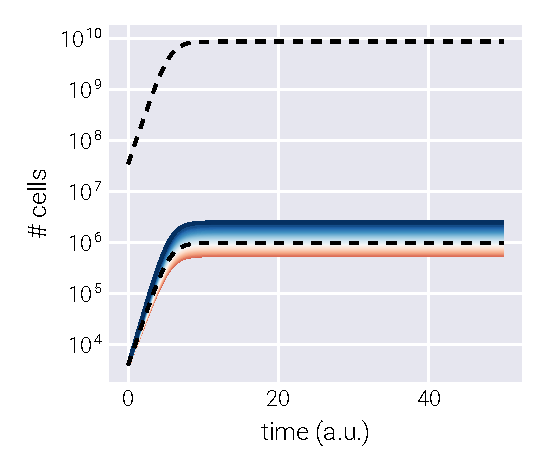
\includegraphics{./figs/figSIX_logistic_growth_01.pdf}

}

\caption{\label{fig-SIX_logistic_growth_01}\textbf{Logistic growth
simulation over single growth cycle}. The dashed line represents the
neutral lineages, with the upper curve being the unlabeled neutral
strain. Color curves represent the genotypes of interest colored by
growth rate relative to the neutral lineage.}

\end{figure}

To simulate multiple growth-dilution cycles, we take the population
composition at the final time point and use it to initialize a new
logistic growth simulation. Figure~\ref{fig-SIX_logistic_growth_02}
shows the resulting number of cells at the last time point of a cycle
over multiple growth-dilution cycles for the genotypes in
@Figure~\ref{fig-SIX_logistic_growth_01}. We can see that the adaptive
lineages (blue curves) increase in abundance, while detrimental lineages
(red curves) decrease.

\begin{figure}

{\centering 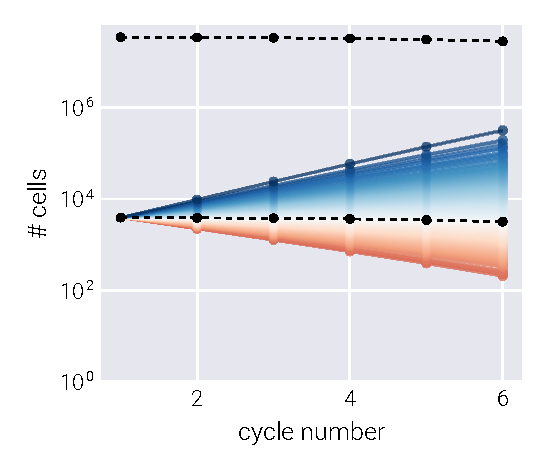
\includegraphics{./figs/figSIX_logistic_growth_02.pdf}

}

\caption{\label{fig-SIX_logistic_growth_02}\textbf{Growth-dilution
cycles for logistic growth simulation}. Each point represents the final
number of cells after a growth cycle for each lineage. Colors are the
same as in Figure~\ref{fig-SIX_logistic_growth_01}.}

\end{figure}

In Section~\ref{sec-fitness_model}, we derive the functional form to
infer the relative fitness of each lineage as
\begin{equation}\protect\hypertarget{eq-logistic_logfreq}{}{
\frac{1}{\tau}\ln \frac{f_{t+1}^{(b)}}{f_{t}^{(b)}} = (s^{(b)} - \bar{s}_t).
}\label{eq-logistic_logfreq}\end{equation}
Figure~\ref{fig-SIX_logistic_growth_03} shows the corresponding log
frequency ratio curves for the logistic growth simulation. The
displacement of these curves with respect to the neutral lineages
determines the ground truth relative fitness value for these
simulations.

\begin{figure}

{\centering 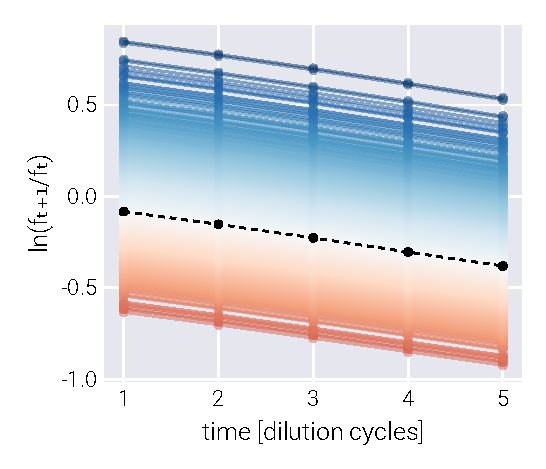
\includegraphics{./figs/figSIX_logistic_growth_03.pdf}

}

\caption{\label{fig-SIX_logistic_growth_03}\textbf{Log frequency ratio
for logistic growth simulations}. The relative distance of the color
curves from the black dashed line determines the relative fitness of
each linage.}

\end{figure}

To simulate the experimental noise, we add two types of noise:

\begin{enumerate}
\def\labelenumi{\arabic{enumi}.}
\tightlist
\item
  Poisson noise between dilutions. For this, we take the final point of
  the logistic growth simulation and sample a random Poisson number
  based on this last point to set the initial condition for the next
  cycle.
\item
  Gaussian noise when performing the measurements. When translating the
  underlying population composition to the number of reads, we can add a
  custom amount of Gaussian noise.
\end{enumerate}

Figure~\ref{fig-SIX_logistic_growth_04} shows the frequency trajectories
(left panels) and log frequency ratios (right panels) for a noiseless
simulation (upper panels) and a simulation with added noise (lower
panels). The noiseless simulation is used to determine the relative
fitness for each of the lineages, which serves as the ground truth to be
compared with the resulting inference.

\begin{figure}

{\centering 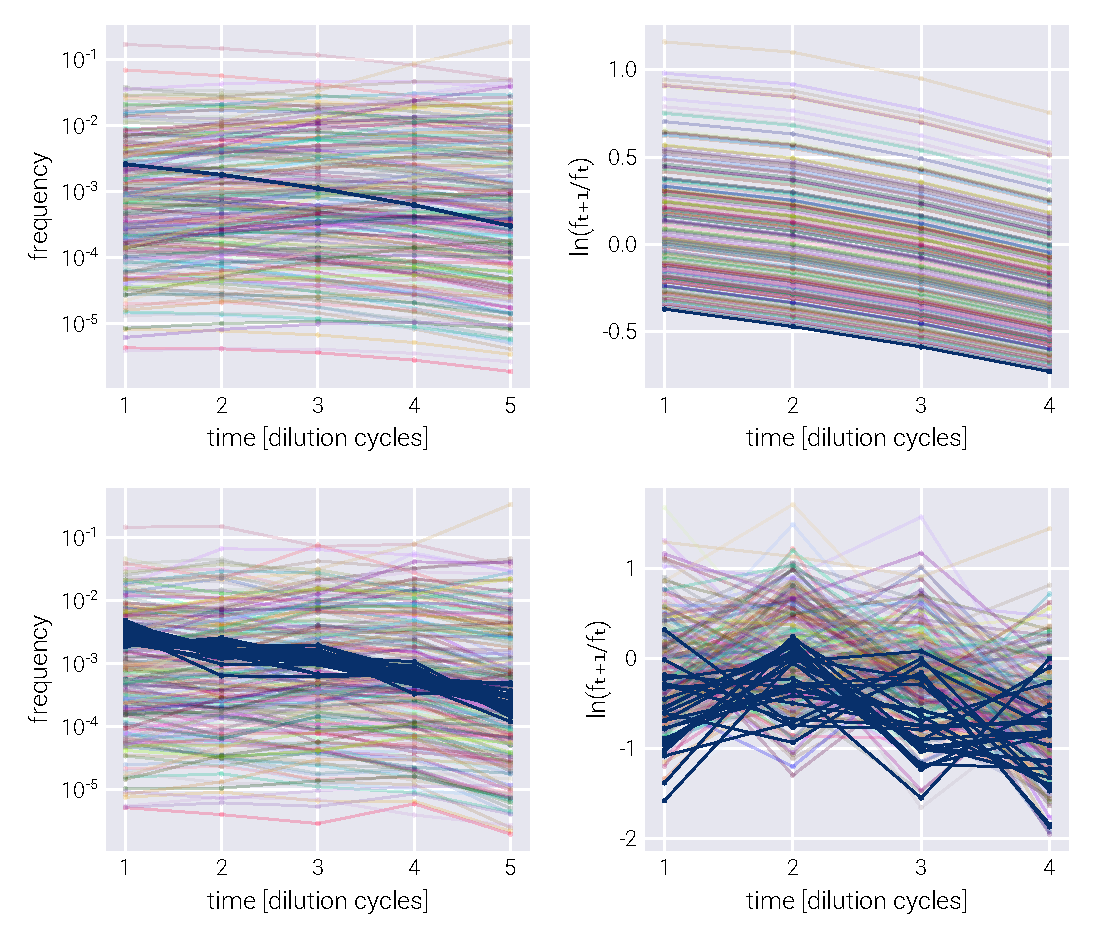
\includegraphics{./figs/figSIX_logistic_growth_04.pdf}

}

\caption{\label{fig-SIX_logistic_growth_04}\textbf{Logistic
growth-dilution simulations with and without noise}}

\end{figure}


% Print supplemental references changing the title
\printbibliography[title={Supplemental References},
segment=\therefsegment, filter=notother]
\end{refsegment}

% \printbibliography


\end{document}
